\hypertarget{die-idee}{%
\section{Die Idee}\label{die-idee}}

Die Idee einer Gärtnerhilfe-Anwendung entstand bereits Anfang April 2020
während des ersten Brainstormings. Im ersten Treffen des Moduls, am
20.04.2020 haben wir vier - Robert Ackermann, Hannes Dröse, Dennis
Krischal und Livia Schumm - uns in einer Projektgruppe zusammengefunden.
Am selben Tag hat unser erstes Webex-Meeting stattgefunden, in dem über
verschiedene Ideen beratschlagt worden ist. Für die Aufgabenstellung mit
dem Motto ``Future Interfaces'' sollen zwei Teilprojekte abgedeckt
werden:

\begin{enumerate}
\def\labelenumi{\arabic{enumi}.}
\tightlist
\item
  Die Entwicklung einer \protect\hyperlink{vision}{Vision}, also die
  Konzeption einer zukunftsweisenden intuitiven Interaktion mit
  digitalen Inhalten und deren Darstellung in Form eines Visionsvideos
\item
  Die Entwicklung eines \protect\hyperlink{prototyp}{Prototyps} dieser
  Vision, sprich die Ausarbeitung einer interaktiven Anwendung
\end{enumerate}

Unsere Projektidee soll also sowohl innovativ als auch in Teilaspekten
umsetzbar sein, jedoch sollten wir uns vorerst mehr auf die Vision als
auf den Prototypen konzentrieren. Es entstand eine Auswahl folgender
Projektthemen:

\begin{itemize}
\tightlist
\item
  Gardening - App zum Gärtnern lernen, unterstützt und lehrt das
  Gärtnern
\item
  Kontaktloses Bezahlen und papierlose Kassenbons
\item
  Verwaltung - Online Identitätsfeststellungen, Digitale Formulare
\item
  Antlitzdiagnostik - Apps analysieren den Gesundheitszustand,
  appgestützte Ferndiagnose mit Ärzten
\end{itemize}

Der gemeinsame Favorit hat sich im Gespräch jedoch schnell abgezeichnet
und nach einer kurzen Themenabstimmung mit den betreuenden Dozenten hat
die Richtung in den Gardening-Bereich festgestanden.

\hypertarget{recherche}{%
\subsection{Recherche}\label{recherche}}

Der nächste Schritt, nachdem eine Projektrichtung festgesteckt worden
ist, ist die Recherche in diesem Bereich. Im Fall des Gardenings stellen
sich vor allem drei Fragenfelder:

\begin{enumerate}
\def\labelenumi{\arabic{enumi}.}
\tightlist
\item
  Wie sieht Gärtnern aktuell überhaupt aus, woran besteht Bedarf und in
  welche Richtung gehen die Trends der Zukunft?
\item
  Welche Apps, Anwendungen und Projekte gibt es bereits und welche sind
  in der Entwicklung?
\item
  Wie sehen die technischen Möglichkeiten aus? Welche Sensoren,
  Messtechniken o.ä. werden in der Landwirtschaft gebraucht oder sind im
  Garten einsetzbar?
\end{enumerate}

\textbf{Anmerkung:}

Im Folgenden werden nur einige, wesentliche Aspekte dieser Recherche
zusammengetragen, weitere gesammelte Informationen und Artikel finden
sich in unserem Projekt unter den Recherchen im Management-Tool
Asana.\footnote{Allgemeine Recherche und Trends:
  \url{https://app.asana.com/0/1172859492234369/1172897938417709}\\
  Pflanzen Apps:
  \url{https://app.asana.com/0/1172859492234369/1172897938417707}\\
  Sensoren und Messtechnik:
  \url{https://app.asana.com/0/1172859492234369/1172859492239381}}

\hypertarget{trends-und-aktuelle-entwicklung-des-guxe4rtnerns}{%
\subsubsection{Trends und aktuelle Entwicklung des
Gärtnerns}\label{trends-und-aktuelle-entwicklung-des-guxe4rtnerns}}

Dass die Beliebtheit von Gärten, Pflanzen und Natur steigt, merkt schon
alleine, wer sich im eigenen Umfeld umsieht. Zahlreiche Artikel, Blog-
und Social Media-Beiträge zeigen die Trends des \textbf{Urban
Gardening}, des \textbf{Urban Jungles}, des \textbf{DIY} (Do It
Yourself) auf.

Laut dem Zukunftsinstitut\footnote{Artikel ``Die Zukunft ist ein
  Garten'' -
  \url{https://www.zukunftsinstitut.de/artikel/wohnen/die-zukunft-ist-ein-garten/}}
ist die Zahl der Menschen mit Garten oder Balkon in Deutschland zwischen
2007 und 2011 von 50 Millionen auf 55 Millionen gestiegen. Ebenso sinkt
das Durchschnittsalter von Kleingarten-Pächtern stetig ab.\footnote{Artikel
  vom 22.11.2017: ``Blick in die Zukunft: So leben wir im Garten 2030''
  -
  \url{https://taspo.de/kategorien/blick-in-die-zukunft-so-leben-wir-im-garten-2030/}}
Der Trend geht hin zur Begrünung von Gärten, Balkonen, Terrassen, zur
Gründung sowie Nutzung von Gemeinschafts- und Nachbarschaftsgärten --
vor allem bei der naturhungrigen Stadtbevölkerung. Die Gartenbranche
stellt sich langsam auf eine \textbf{neue, jüngere Zielgruppe} ein. Die
steigende Beliebtheit des Gärtnerns jeglicher Art liegt unter anderem im
Ausgleich, den es zum stressigen Stadtalltag bieten kann, aber auch in
seiner guten Vereinbarkeit mit dem Nachhaltigkeits-Trend. Verschiedene
Faktoren lassen haufenweise individuelle und clevere Ansätze entstehen.
Die Nachfrage nach Bio-Produkten und Nutzpflanzen und dafür möglichst
einfachen aber autonomen Systemen ist groß.

Der Platzmangel in Städten verlangt z.B. nach vertikalen Lösungen:

\begin{itemize}
\tightlist
\item
  ``Pflanzetageren'': Versetzt angeordnete, kleeblattförmige Gefäße, die
  sich hoch stapeln lassen
\item
  ``Minigarden'': vertikales Pflanzsystem, Begrünung von Wänden oder
  kompletter Balkonbrüstung
\item
  ``Skyplanter'': Pflanzen wachsen in einer Art umgedrehtem Blumentopf
  von der Decke herab nach unten
\end{itemize}

Doch nicht nur das Interesse in Richtung zurück zum Ursprünglichen --
zur Natur -- ist groß, sondern auch innovative, konnektive Lösungen sind
gefragt, die das Leben in Haus und Garten durch \textbf{smarte Technik}
vereinfachen. In seinem Vortrag auf dem DIY Garden Summit 2017 in
Berlin\footnote{Artikel vom 22.11.2017: ``Blick in die Zukunft: So leben
  wir im Garten 2030'' -
  \url{https://taspo.de/kategorien/blick-in-die-zukunft-so-leben-wir-im-garten-2030/}}
erklärt Christian May, Geschäftsführer von Kärcher, wie ein Tag im
Garten des Jahres 2030 aussehen könnte:

\begin{quote}
Während eines gemütlichen Frühstücks in der Sonne auf meiner Terrasse
fällt mein Blick auf den Grill: Ihn umgeben unschöne Überbleibsel vom
gestrigen Grillfest. Doch dem Hochdruckreiniger fehlt der spezielle
Aufsatz für Rußflecken. Schnell ist die passende Vorlage gefunden und
kurz darauf druckt der 3D-Drucker den fehlenden Aufsatz aus und die
Arbeit kann beginnen. Da ich nun schon einmal im Garten bin, kümmere ich
mich auch gleich um meine Blumenbeete. Während ich mich umschaue, zeigen
mir einzelne Pflanzen auf meiner Smart-Brille an, dass sie nicht genug
Sonne bekommen und umgepflanzt werden müssen. Am Nachmittag ist es Zeit
für meinen Videokurs zum Thema Pflanzen, Pflegen und Ernten seltener
Gemüsesorten -- meinem Steckenpferd. Meine Expertise auf dem Gebiet
teile ich gerne und inzwischen lauschen meinen interaktiven
wöchentlichen Livestreams interessierte Hobbygärtner und Landwirte aus
Kanada, Südafrika und Japan, die mich wiederum an ihrem Wissen teilhaben
lassen. Am Abend bin ich mit Freunden zum Abendessen verabredet. Während
der Vorspeise bekomme ich eine Nachricht: Die Sonne brannte heute den
ganzen Tag und meine Pflanzen sind durstig. Jetzt, wo es langsam
schattiger wird, ist der perfekte Zeitpunkt, meine Rosen zu bewässern.
Per Knopfdruck bestätige ich, das automatische Bewässerungssystem legt
los und ich kann mich wieder in Ruhe meiner Vorspeise widmen.
\end{quote}

Aus diesem Beispiel gehen gleich mehrere mögliche Zukunftsaspekte
hervor:

\begin{itemize}
\tightlist
\item
  konnektive Lösung mittels 3D Drucker zum Drucken von Ersatzteilen und
  Hilfsmitteln
\item
  Smart-Brille erfasst Umgebungs- und Pflanzenzustand (Bewässerung,
  Sonnenbelichtung etc.)
\item
  Austausch von Wissen über Vernetzungskomponente
\item
  smarte Auswertung verschiedener, zusammenspielender Informationen
  (Gießzustand der Pflanzen plus Ermittlung des optimalen Zeitpunktes)
\item
  automatisierte Systeme zur Versorgung (in dem Fall Bewässerungsanlage
  per Knopfdruck)
\end{itemize}

\hypertarget{technisch-relevante-daten-der-pflanzenwelt}{%
\subsubsection{Technisch relevante Daten der
Pflanzenwelt}\label{technisch-relevante-daten-der-pflanzenwelt}}

Aufwendige und smarte Technik wird zurzeit vor allem im
Großanbau-Rahmen, also in der Landwirtschaft, eingesetzt. Das
\textbf{Digital Farming} hat sowohl in der Tierindustrie als auch im
Anbau Einzug gehalten - die Landschaft steckt mitten drin in der
Digitalisierung, neudeutsch: \textbf{``Smart Farming''}.\footnote{vgl.
  Artikel vom 10.11.2019, Link:
  \url{https://www.deutschlandfunk.de/digitalisierung-der-landwirtschaft-daten-saeen-daten-ernten.740.de.html?dram:article_id=462957}}
Für die Landwirte bietet das sowohl Vor- als auch Nachteile, im Hinblick
auf ein interaktives Gardening-Projekt sind aber vor allem die
technischen Möglichkeiten relevant und was man aus ihrem Einsatz in der
Landwirtschaft lernen kann. Allgemein dient Smart Farming der
Optimierung von Planung, Effizienz und Ertrag.

\textbf{Precision Farming:} Komplettangebote von IT-Konzernen zur
Optimierung der Pflanzen für die Weiterverabeitung (z.B. Berechnung des
Abstands zwischen Pflanzen, damit sie die richtige Größe bekommen).
Mithilfe von Sensoren auf dem Feld und in den Böden, vernetzten
Maschinen und entsprechenden Analyse-Softwares, die zusätzlich benötigte
Daten, wie Geo- und Wetter-Analysen, mit einbeziehen wird für eine
großflächig abdeckende, informationstechnische Infrastruktur gesorgt.
\footnote{vgl. Artikel vom 10.11.2019, Link:
  \url{https://www.deutschlandfunk.de/digitalisierung-der-landwirtschaft-daten-saeen-daten-ernten.740.de.html?dram:article_id=462957}}

Der \textbf{Einsatz von Drohnen} und \textbf{Auswertung von
Satellitenbilder} hilft bei der Planung von Aussaat, Pflege und Ernte:

\begin{itemize}
\tightlist
\item
  BayWa-Drohnen ermöglichen beispielweise eine automatische
  Schädlingserkennung und -bekämpfung.\footnote{vgl. Artikel vom
    23.06.2017, Link:
    \url{https://biooekonomie.de/digitale-landwirtschaft-it-fuer-acker-und-stall}}
\item
  Das Copernicus-Programm beinhaltet zum Beispiel
  Satellitenfernerkundungssysteme, das verschiedene Daten
  (Pflanzenstrukturen und Bodenbewegungen, Landbedeckung und
  Landnutzung) zum optimalen Düngermanagement sammelt.
\item
  Positionsgenaue Regenradar-Apps dienen der optimalen Bewässerung von
  Feldern.\footnote{vgl. Artikel vom 23.06.2017, Link:
    \url{https://biooekonomie.de/digitale-landwirtschaft-it-fuer-acker-und-stall}}
\end{itemize}

\textbf{Farm Managment}: Eine datengestützte, automatische Dokumentation
spart Zeit. In Zukunft soll sogar nur noch geringfügig menschliche
Arbeit vonnöten sein indem Maschinen direkt mit Maschinen
kommunizieren.\footnote{vgl. Artikel vom 21.07.2020, Link:
  \url{https://www.computerwoche.de/a/was-sie-ueber-landwirtschaft-4-0-wissen-muessen,3544215}}

Herausforderungen für die IT stellen sich hauptsächlich durch die
Verwaltung enormer Datenmengen und deren Austausch über das mobile Netz.
Gerade in den ländlichen Regionen, in denen Landwirtschaft stattfindet,
stellt eine nicht vorhandene Flächendeckung von Netzzugang mit hoher
Bandbreite\footnote{vgl. Artikel vom 23.06.2017, Link:
  \url{https://biooekonomie.de/digitale-landwirtschaft-it-fuer-acker-und-stall}}
teilweise ein Problem dar.

Zusammenfassend kann man aus dem Beispiel der Landwirtschaft folgende
Daten als relevant für jegliche Form von Pflanzenanbau ableiten:

\begin{itemize}
\tightlist
\item
  Bodenbeschaffenheit (Zusammensetzung, Nährstoffe, Durchlässigkeit,
  Bodenfeuchtigkeit)
\item
  Zustandsanalysen (Größe, Abstände, Schädlinge)
\item
  Wetterdaten (Belichtung, Bewässerung, Unwetter)
\item
  Geo-Daten (Pflanzenstrukturen und Bodenbewegungen, Landbedeckung und
  Landnutzung)
\item
  Pflanzendaten (Wissen zur Pflanzenart und ihren Bedürfnissen)
\end{itemize}

Um diese Daten zu gewinnen bedarf es verschiedener Quellen. Für präzise,
lokale Daten bedarf es oft festinstallierter Hardware (Sensoren), die
sich wohl nicht bewährt hat.\footnote{vgl. Artikel vom 10.11.2019, Link:
  \url{https://www.deutschlandfunk.de/digitalisierung-der-landwirtschaft-daten-saeen-daten-ernten.740.de.html?dram:article_id=462957}}
Der Trend entwickelt sich immer mehr in Richtung mobiler Analysen über
Roboter und Drohnen. Je größer der Anbau-Rahmen desto mehr lohnen sich
logischerweise großangelegte, technische Systeme. Die Frage ist nun wie
sich solche Systeme flexibel genug an den Privatgebrauch und dessen
technische Gegebenheiten anpassen lassen, um auch für diese Zielgruppe
lohnenswert zu sein.

Mit dieser Frage beschäftigen sich auch Garten-Dienstleister,
Unternehmer und Start-Ups - welches Angebot dafür bereits besteht
behandelt der nächste Abschnitt.

\hypertarget{bereits-bestehende-projekte}{%
\subsubsection{Bereits bestehende
Projekte}\label{bereits-bestehende-projekte}}

Interaktive, technische Anwendungen im Bereich des Gardening gibt es
auch für die Otto-Normalverbrauchenden bereits reichlich in
verschiedenen Ausführungen, wenn auch nicht in so ausgefeiltem Stil wie
in der Landwirtschaft. Meist greifen sie eine unterschiedliche Auswahl
an den im vorigen Abschnitt erläuterten Aspekten auf. Man kann sie
anhand der Funktionalität jedoch grob unterteilen in:

\begin{itemize}
\tightlist
\item
  visualisierende Planungs-Tools
\item
  einfache Erinnerungs-Anwendungen
\item
  Pflanzenerkennungs-Apps und
\item
  smarte, teils automatisierte Beete.
\end{itemize}

Produkte und Projekte gibt es dazu viele. Im Folgenden werden zur
Verdeutlichung jeweils einige Beispiele vorgestellt.

\hypertarget{visualisierungs-software}{%
\paragraph{Visualisierungs-Software}\label{visualisierungs-software}}

\begin{itemize}
\tightlist
\item
  \textbf{Garten-Planer:} Beispiel ``Home Design 3D Outdoor \&
  Garden''\footnote{Link:
    \url{https://en.homedesign3d.net/2018/10/09/update-v4-2-outdoor-garden/}}
  -- Eine App, die einen virtuellen Rundgang im eigenen Garten
  ermöglicht.
\item
  \textbf{Beet-Planer:} Beispiel ``Alphabeet''\footnote{Link:
    \url{https://www.alphabeet.org/}} -- Wer sich hier anmeldet, kann
  zunächst einmal seine Beete digital anlegen. Je nach Größe wird
  vorgeschlagen, welche Pflanzen wo angebaut werden sollten und auch
  zueinander passen. Ist das Beet fertig geplant, wird automatisch eine
  Aufgabenliste erzeugt, die per Mail an die täglich nötigen Arbeiten
  erinnert und online bei Erledigung abgehakt werden können: Tomaten
  ausgeizen, Unkraut entfernen, Stecklinge ziehen, Möhren abdecken,
  Gießen und vieles mehr.
\end{itemize}

Hierbei stehen also drei Aspekte im Vordergrund: Planen, Umsetzen und
Lernen anhand der Infobibliothek.

\hypertarget{gieuxdf--und-pflegeerinnerungs-apps}{%
\paragraph{Gieß- und
Pflegeerinnerungs-Apps}\label{gieuxdf--und-pflegeerinnerungs-apps}}

Dabei handelt es sich um reine Organisations-Tools, in denen man
Aufgaben verwalten und Erinnerungen erstellen kann. Sie ermöglichen
außerdem Zugriff auf Datenbanken, die dem User nützliche Informationen
zu seinen Pflanzen bieten.

Beispiele für diese Art App sind:

\begin{itemize}
\tightlist
\item
  Gardenia (iPhone // Android)
\item
  myPlants - Manage Tool und Reminder (iPhone // Android)
\item
  PeppyPlant (iPhone)
\item
  Happy Plant (iPhone)
\item
  Plant Watering Reminder (iPhone)
\item
  Plant Diary (Android)
\end{itemize}

\hypertarget{pflanzenerkennungs-apps}{%
\paragraph{Pflanzenerkennungs-Apps}\label{pflanzenerkennungs-apps}}

Die Hauptfunktion solcher Apps ist die Erkennung von Pflanzen anhand von
Fotos. Sie verfügen ebenso über eine Pflanzenenzyklopädie, aus der der
User weitere Informationen erlangen kann. Außerdem wird ein Austausch
über eine Community ermöglicht, über die die App hauptsächlich
funktioniert -- je größer und aktiver die Community desto größer die
Datenbank, desto präziser also auch die Bilderkennung.

Beispiele für diese Art App sind:

\begin{itemize}
\tightlist
\item
  PictureThis\footnote{Link: \url{https://www.picturethisai.com/}}
\item
  PlantNet\footnote{Link: \url{https://plantnet.org/en/}}
\item
  PlantSnap\footnote{Link: \url{https://www.plantsnap.com/}}
\item
  Garden Flower Identification\footnote{Link:
    \url{https://apps.apple.com/us/app/garden-flower-identification-plant-identifier-free/id1128290219}}
\end{itemize}

\hypertarget{smarte-automatisierte-beete}{%
\paragraph{Smarte, automatisierte
Beete}\label{smarte-automatisierte-beete}}

Beispiel: Start-Up \textbf{IP Garten}\footnote{Link:
  \url{https://ipgarten.de/}}

Hierbei handelt es sich um ein Dienstleistungsunternehmen, bei dem man
Beete buchen kann. Diese werden live überwacht mittels Kameras und
Feuchtigkeitssensoren. Interagiert werden kann von zuhause aus über eine
virtuelle Welt auf dem Computer. Eine ferngesteuerte Bewässerung ist für
den Kunden möglich, alle weiteren Gärtner-Leistungen werden hinzugebucht
und von Mitarbeitern durchgeführt. Der Ertrag des gebuchten Beetes kann
nach der Ernte abgeholt oder geliefert werden.

Beispiel: \textbf{Urban connected Gardening mit smartem
Hochbeet}\footnote{Quelle:
  \url{https://computerwelt.at/news/iot-macht-aus-hochbeeten-smartbeete/}}

Dieses Projekt entstand durch eine Kooperation aus ``Smartgreen
Solutions'' und ``T-Mobile Austria''. Im Vergleich zum ersten Beispiel
ist dieses Smartbeet-System autark. Es wird mit Regenwasser und
Solarenergie betrieben. Ausgestattet mit Sensoren, wird eine Vielzahl an
Faktoren gemessen: Temperatur, Feuchtigkeit, Sonneneinstrahlung,
Stromverbrauch, Wasserdurchfluss etc. Außerdem hat Smartgreen Solutions
eigens eine elektronische Steuereinheit entwickelt, um das Beet
automatisch reagieren zu lassen. Diese Steuereinheit sendet zudem Daten
über T-Mobiles IoT-Box an die Smartgreen-Cloud, wodurch der User sie auf
der eigenen App abrufen und kontrollieren kann. Die IoT-Box wiederum
versorgt die Steuerung mit Daten, wie zum Beispiel Wetterdaten.

\textbf{Smart und automatisiert} bedeutet also immer, dass eine gewisse
Hardware-Ausstattung vonnöten ist und muss lokal installiert sein. Je
aufwendiger die Ausstattung, desto mehr Möglichkeiten ergeben sich für
das Beet.

\textbf{Anmerkung:}

Eine zusammengetragene Liste weiterer Crowdfunding Projekte zu dem Thema
findet sich in unserem Projekt unter den Recherchen im Management-Tool
Asana.\footnote{Link:
  \url{https://app.asana.com/0/1172859492234369/1172957097729748}}

\hypertarget{festlegung-des-projektrahmens}{%
\subsection{Festlegung des
Projektrahmens}\label{festlegung-des-projektrahmens}}

Aufgrund der Fülle an Themengebieten und bereits existierenden
Projekten, soll nun die Vision und ihr potenzieller Wirkungsraum von den
recherchierten Projekten abgegrenzt werden.

Es soll sich um kein landwirtschaftliches Projekt, sondern um eine
Anwendung für den Privatgebrauch handeln. In diesem Rahmen soll sie
jedoch so universell wie möglich einsetzbar sein. Es stellt sich also
die Frage, wie sich möglichst flexible, mobile Systeme mit einer
möglichst präzisen, lokalen Datengewinnung gestalten lassen. Sind
Sensoren unablässig oder lassen sie sich beispielsweise durch
Scan-Geräte ersetzen? Was können Scanner zurzeit und was möglicherweise
in der Zukunft? Und welche Geräte sind in welchem Rahmen einsetzbar?

Der erste Schritt, um vor dem Hintergrund dieser Fragestellungen den
Projektrahmen zu finden, ist die Erstellung von Zielgruppen Personas.
Auf deren Basis können dann die Anforderungen für das Visions-Produkt
entstehen.

\hypertarget{erstellen-von-zielgruppen-personas}{%
\subsubsection{Erstellen von Zielgruppen
Personas}\label{erstellen-von-zielgruppen-personas}}

\hypertarget{zielgruppe-allgemein}{%
\paragraph{Zielgruppe allgemein}\label{zielgruppe-allgemein}}

Die allgemeine Zielgruppe umfasst Privatpersonen, die Interesse am
Gärtnern haben. Dadurch, dass Gardening ein Trend-Thema ist, handelt es
sich also um eine relativ große, breit gefasste Zielgruppe. Im Fokus
soll jedoch das Gärtnern Lernen stehen. Dies soll durch Technik
unterstützt werden, die beim User bereits vorhanden ist. Der Prozess des
Lernens soll dabei durch angeleitete Tätigkeiten am realen Objekt
geschehen. Es handelt sich also um kein virtuelles Lerntool.

\hypertarget{beispiel-personas}{%
\paragraph{Beispiel-Personas}\label{beispiel-personas}}

Die allgemeine Zielgruppe könnte Personen mit folgenden Steckbriefen
enthalten:

\textbf{Jonas:}

\begin{itemize}
\tightlist
\item
  24 Jahre alt
\item
  Student
\item
  interessiert an Nachhaltigkeit und grünen Themen
\item
  in der Stadt aufgewachsen
\item
  bisher keinen Bezug zum Gärtnern oder zu Pflanzen, aber Sehnsucht nach
  Grün und Gartenidylle
\item
  hat also kaum Erfahrung damit, möchte es aber Lernen und Ausprobieren
\item
  wenn es ihm gefällt, macht er vielleicht mehr in die Richtung
\item
  ist technisch komplett ausgestattet mit diversen gängigen Geräten
  (mobil, aber auch stationäre, smarte Assistenten)
\end{itemize}

\textbf{Martina:}

\begin{itemize}
\tightlist
\item
  26 Jahre alt
\item
  hat bereits Erfahrung mit Pflanzen
\item
  möchte mehr lernen und Garten-Profi werden
\end{itemize}

\textbf{Mike:}

\begin{itemize}
\tightlist
\item
  34 Jahre alt
\item
  begeisterter Gärtner mit sehr großem Garten und vielen Pflanzen
\item
  kann sich gar nicht wirklich um alles kümmern und braucht Hilfe dabei
\end{itemize}

Der Fokus für das Visionsvideo soll vor allem auf Jonas festgelegt sein.

\hypertarget{features1}{%
\subsubsection{Features - Vision vs.~grobe Richtung
Prototyp}\label{features1}}

Aus der Zielgruppe ergibt sich die Schlussfolgerung ein möglichst
Hardware-armes Produkt zu entwickeln, das universell für viele Nutzer
einsetzbar ist. Das heißt auf technische Geräte zu setzen, die bereits
in jedem Haushalt vorhanden sind. Zurzeit ist dies unbestritten das
Smartphone, aber auch erweiternde SmartHome-Geräte halten immer mehr
Einzug. Auch wenn sich User Interface und technische Ausstattung stetig
wandeln, wird uns auch in Zukunft das Smartphone weiter begleiten. Auf
diese Annahme setzt Grüni. Die folgende Grafik zeigt den Stand von
definierten Soll-Anforderungen vom 29.04.2020 (vgl. mit späterer
\protect\hyperlink{ux5cux23ux5cux23Interaktionsgestaltung}{Darstellung
im Video} sowie \protect\hyperlink{ux5cux23Umsetzung}{Umsetzung beim
Prototypen}):

\begin{figure}
\centering
\includegraphics{img/Projektthema.jpg}
\caption{Grafik `Vision vs.~Prototyp'}
\end{figure}

Zusätzlich zu der technischen \textbf{Ausstattung zur Analyse} gibt es
ebenfalls Hardware zur \textbf{Versorgung} der Pflanzen. Dies soll mit
der Anwendung Grüni zwar möglich sein, aber freiwillig, da weitere
Geräteinstallationen dafür nötig sind. Der Lern- und Informations-Aspekt
stehen im Vordergrund.

Für den Prototypen war jedoch bereits zu diesem Zeitpunkt klar, dass wir
nicht auf externe Sensoren verzichten werden können und auch der
Wirkungsraum spezifisch eingegrenzt sein wird. Dazu allerdings erst mehr
unter dem Punkt \protect\hyperlink{prototyp}{Prototyp}.

\hypertarget{herausforderungen-in-der-projektfindungssphase}{%
\subsection{Herausforderungen in der
Projektfindungssphase}\label{herausforderungen-in-der-projektfindungssphase}}

Eine große Herausforderung hat in der Masse an Recherche-Material
bestanden, welches durchgelesen und aussortiert werden musste. Aus
dieser Flut hat sich die genaue Definition, was denn nun genau mit der
Grüni Anwendung erreicht werden soll, als schwierig herausgestellt.
Ebenso ist die klare Abgrenzung zu den vielen anderen Projekten schwer
gefallen.

\hypertarget{vision}{%
\section{Die Vision}\label{vision}}

Der Weg durch die Projektfindungsphase führt nun also zur Anwendung
``Grüni''. Grüni ist ein universelles Hilfstool für Pflanzen, welches im
Haus oder Garten Einsatz findet. Sie beherrscht sehr umfangreiche
Analysen, Simulationen und Funktionalitäten rund um das Gärtnern. Dabei
ist die Größe des Topfes, Beetes oder Gartens sowie die Auswahl der
Geräte, auf denen die App funktioniert, komplett variabel und frei. Es
kommen sehr ausgefeilte Arten der holografischen Visualisierung zum
Einsatz, bis hin zu einem personifizierten Gartengehilfen -- PLANT-E.
Wobei PLANT-E selbst keine Arbeiten verrichten kann, sondern als
holografischer Assistent den Nutzer vor allem durch Prozesse (Eintopfen,
Umtopfen etc.) führt oder Erinnerungen gibt.

\hypertarget{geplante-eigenschaften-und-features-der-zukunftsvision}{%
\subsection{Geplante Eigenschaften und Features der
Zukunftsvision}\label{geplante-eigenschaften-und-features-der-zukunftsvision}}

\begin{itemize}
\tightlist
\item
  Geräteunabhängigkeit - App läuft auf stationären Geräten (z.B.
  Echo-Dots), mobilen Endgeräten (z.B. Smartphone, Tablet)-
  Geräteübergreifend

  \begin{itemize}
  \tightlist
  \item
    Messungen von einem Gerät (steht bei den Pflanzen)
  \item
    Mitteilung des Nutzers über ein anderes Gerät (welches ihm gerade am
    nächsten ist)
  \end{itemize}
\item
  Nutzung in verschiedensten Umgebungen

  \begin{itemize}
  \tightlist
  \item
    sowie innerhalb als auch außerhalb des Hauses
  \item
    ein paar Töpfe / ein Beet/ ein ganzer Garten
  \end{itemize}
\item
  Analyse der Umgebung via Scan

  \begin{itemize}
  \tightlist
  \item
    geeignete Orte für die Pflanzen finden anhand ihrer Art und deren
    Bedürfnissen
  \end{itemize}
\item
  Beetplanung / Simulation des Pflanzenwachstums innerhalb einer
  gegebenen Umgebung

  \begin{itemize}
  \tightlist
  \item
    holografische Visualisierung von Pflanzen an entsprechenden Stellen
    inklusive Simulation wie sich die Pflanze dort entwickeln würde
  \end{itemize}
\item
  Pflanzenerkennung

  \begin{itemize}
  \tightlist
  \item
    Klassifizierung von Pflanzen und Samen via Scan
  \end{itemize}
\item
  Bereitstellung von Informationen zur Pflanze
\item
  Bestimmung des Zustands der Pflanze

  \begin{itemize}
  \tightlist
  \item
    Alter, Bewässerung, Bodenzustand, Lichtverhältnisse, Reifegrad der
    Früchte usw.
  \end{itemize}
\item
  Visualisierung dieser Zustandsinformationen (z.B. mit einer Gieß- bzw.
  Bewässerungsanzeige)

  \begin{itemize}
  \tightlist
  \item
    holografisch, symbolisch, auditiv
  \end{itemize}
\item
  Erinnerungsfunktion z.B. ans Gießen, Umtopfen, Rausstellen (z.B. in
  Form von PLANT-E)
\item
  Vorschläge und Produktempfehlungen

  \begin{itemize}
  \tightlist
  \item
    entsprechend der aktuellen Bedürfnisse der Pflanzen werden die
    benötigten Tools und Komponenten direkt zur Bestellung angeboten
  \end{itemize}
\item
  der Lehrmeister \textbf{PLANT-E}

  \begin{itemize}
  \tightlist
  \item
    Personifizierung des Computers für den Menschen
  \item
    Tipps Erinnerungen und Co.~werden dem Nutzer über PLANT-E mitgeteilt
  \end{itemize}
\item
  Fingerabdruck-Scan

  \begin{itemize}
  \tightlist
  \item
    zum Autorisieren von Transaktionen
  \end{itemize}
\item
  Gestenerkennung

  \begin{itemize}
  \tightlist
  \item
    Greifen (zum Auswählen), leichtes Nicken, Rahmen für einen
    Schnappschuss setzen
  \end{itemize}
\item
  Community-Komponente / Sharing-Funktion

  \begin{itemize}
  \tightlist
  \item
    Möglichkeit die eigenen Pflanzen mit den Freunden zu teilen,
    fotobasiert
  \end{itemize}
\end{itemize}

\hypertarget{videovorbereitungen}{%
\subsection{Videovorbereitungen}\label{videovorbereitungen}}

\hypertarget{drehbuch}{%
\subsubsection{Drehbuch}\label{drehbuch}}

Der erste Schritt zur Filmkreation ist die Überlegung gewesen, welche
Aspekte der Vision Grüni als Produkt dargestellt werden sollen. Da der
Umfang der Visionsidee sehr groß und variabel ist, ist die Handlung auf
eine bestimmte Zielgruppe festgelegt worden - die im festgelegten
Projektrahmen definierte Zielgruppe ``Jonas''. Schon bei der ersten
Version des Drehbuches ist direkt klar geworden, wer die Rolle dieser
Zielgruppe treffen würde und so hat die Wahl unseres Hauptdarstellers
schnell festgestanden. In diesem Zuge ist der Name ``Jonas'' auf
``Christian'' geändert worden. Christian startet entsprechend seiner
Persona mit keinerlei Grundwissen, kommt zufällig an Gärtner-Material
und wird daraufhin auf die Anwendung gestoßen.

Dramaturgisch findet die Entwicklung gleichermaßen zwischen Mensch und
App statt. Die Darstellung der App geschieht hauptsächlich über PLANT-E,
der dabei wie ein virtueller Lehrer ist und Christian das Gärtnern im
Rahmen seiner Ausstattung und Möglichkeiten vorort beibringen soll.

Inspiriert war die Idee PLANT-Es ursprünglich vom Roboter WALL·E aus dem
Film ``WALL·E -- Der Letzte räumt die Erde auf'', daher auch der Name.
Anfänglich sollte PLANT-E auch in seiner Art der Kommunikation an WALL·E
angelehnt sein, sprich er sollte möglichst wenig sprechen, sondern
hauptsächlich über Gestik und Mimik kommunizieren. Realistisch war dies
für die Umsetzung seiner Funktion als Ratgeber und Lehrmeister
allerdings nicht, darum ist die Entscheidung doch auf Dialoge gefallen.

Weitere im Verlauf der Entwicklung für die Handlung festgelegte Aspekte
des Filmes:

\begin{itemize}
\tightlist
\item
  (Alexa) Echos = Analysegerät (Scan)

  \begin{itemize}
  \tightlist
  \item
    Wohnung und Balkon bei Christian
  \item
    Kommunikation zwischen Christian und Schwester
  \end{itemize}
\item
  Handy = Projektor

  \begin{itemize}
  \tightlist
  \item
    Andeutung von Variabilität durch Nachbarsgärten -- Andeutung einer
    Community durch Posts
  \end{itemize}
\end{itemize}

Die Endfassung des Drehbuches findet sich im
\protect\hyperlink{anhang}{Anhang}.\footnote{Alle Versionen des
  Drehbuches finden sich im Google-Drive Ordner unter dem Link:
  \url{https://drive.google.com/drive/folders/1toOwAzorJRI8cY0EzBIM56n-LDfFUXsK}}

\hypertarget{interaktionsgestaltung-und-ui-design}{%
\subsubsection{Interaktionsgestaltung und
UI-Design}\label{interaktionsgestaltung-und-ui-design}}

Bei der Entwicklung des Drehbuches wurde bereits schnell deutlich, dass
die Interaktionsgestaltung im Fokus der Handlung stehen sollte. Wie die
Features der Vision in der Interaktion aussehen, zeigt sich in den
folgenden Designentwurf-Skizzen (Stand 26.05.2020) zur Umsetzung in den
Szenen:

\hypertarget{szene-2}{%
\paragraph{Szene 2}\label{szene-2}}

\begin{itemize}
\tightlist
\item
  Verarbeitung von Sprachbefehlen
\item
  Scannen des Raums, Identifizierung der Gegenstände → Erkennung von
  Anzuchtkasten und Samen:

  \begin{itemize}
  \tightlist
  \item
    Stil-Inspiration: \url{https://www.youtube.com/watch?v=3HbkcRAQhew}
  \end{itemize}
\end{itemize}

\begin{figure}
\centering
\includegraphics{img/UI/Raumscan1.png}
\caption{UI Raumscan 1}
\end{figure}

\begin{figure}
\centering
\includegraphics{img/UI/Raumscan2.png}
\caption{UI Raumscan 2}
\end{figure}

\begin{figure}
\centering
\includegraphics{img/UI/Raumscan3.png}
\caption{UI Raumscan 3}
\end{figure}

\begin{itemize}
\tightlist
\item
  Visualisierung der Pflanzen:
\end{itemize}

\begin{figure}
\centering
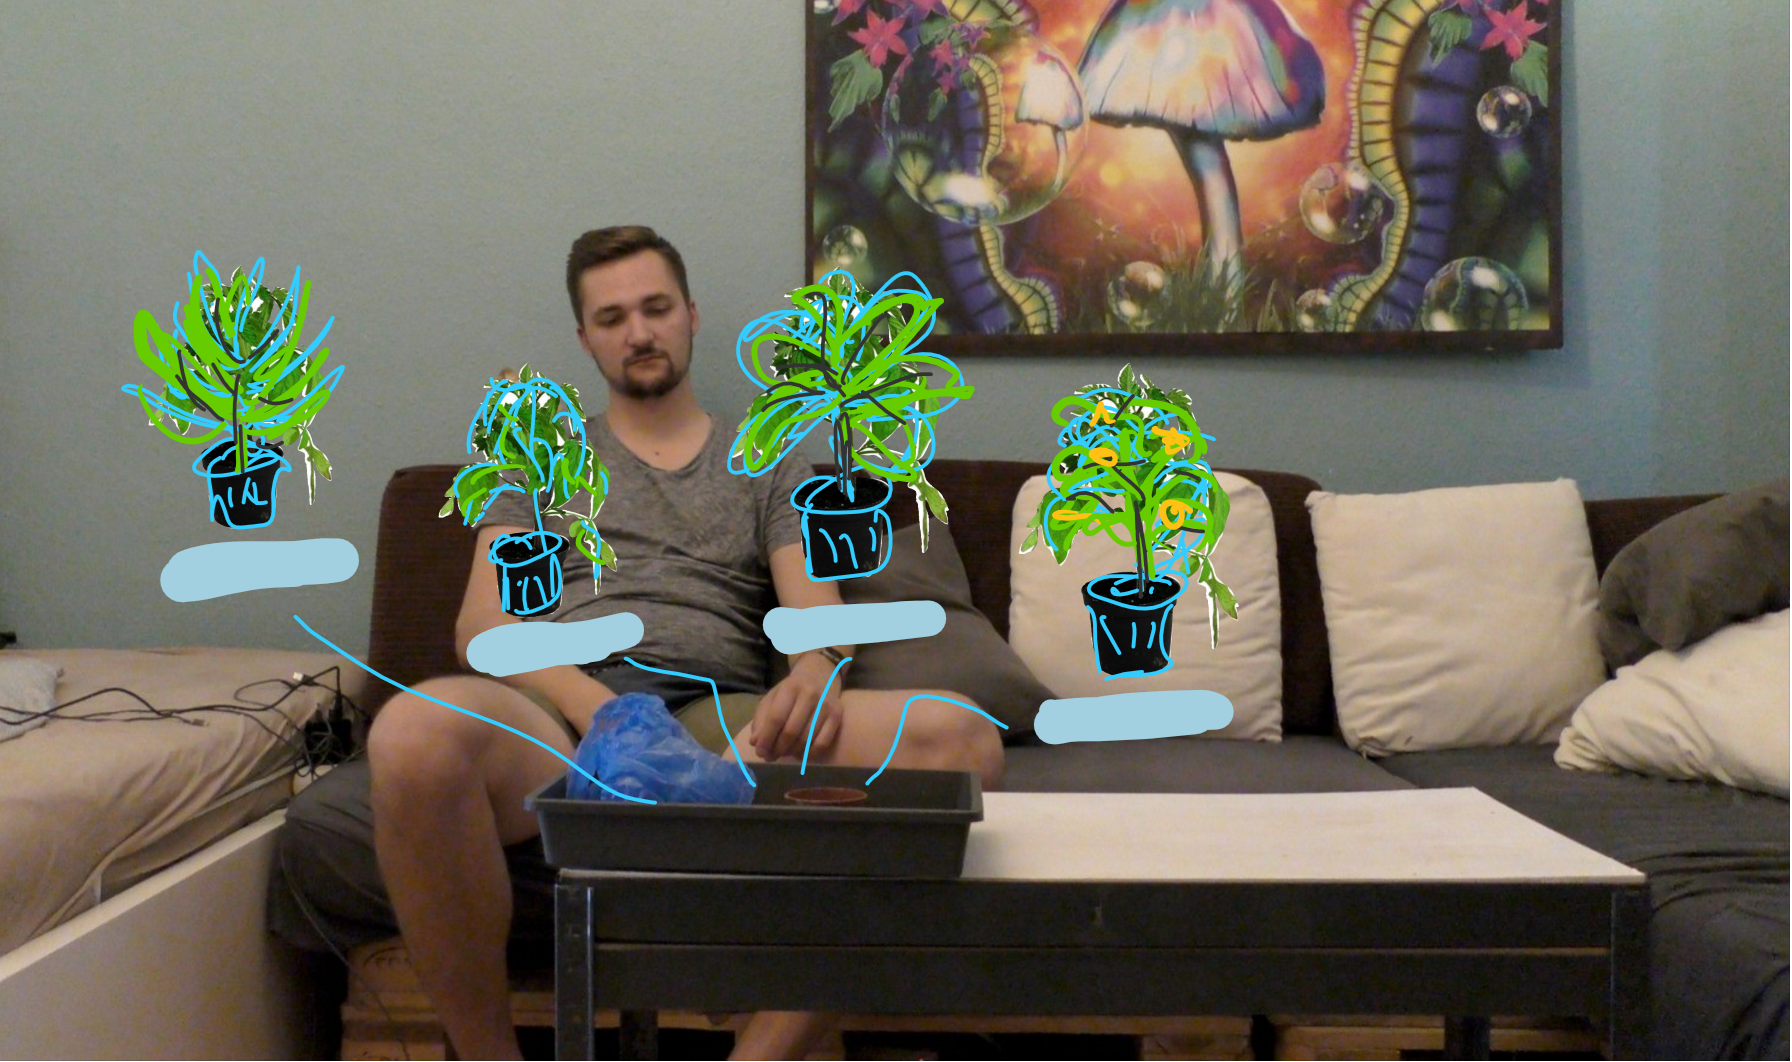
\includegraphics{img/UI/Pflanzenvisualisierung_frontal.png}
\caption{Pflanzenvisualisierung Frontalansicht}
\end{figure}

\begin{figure}
\centering
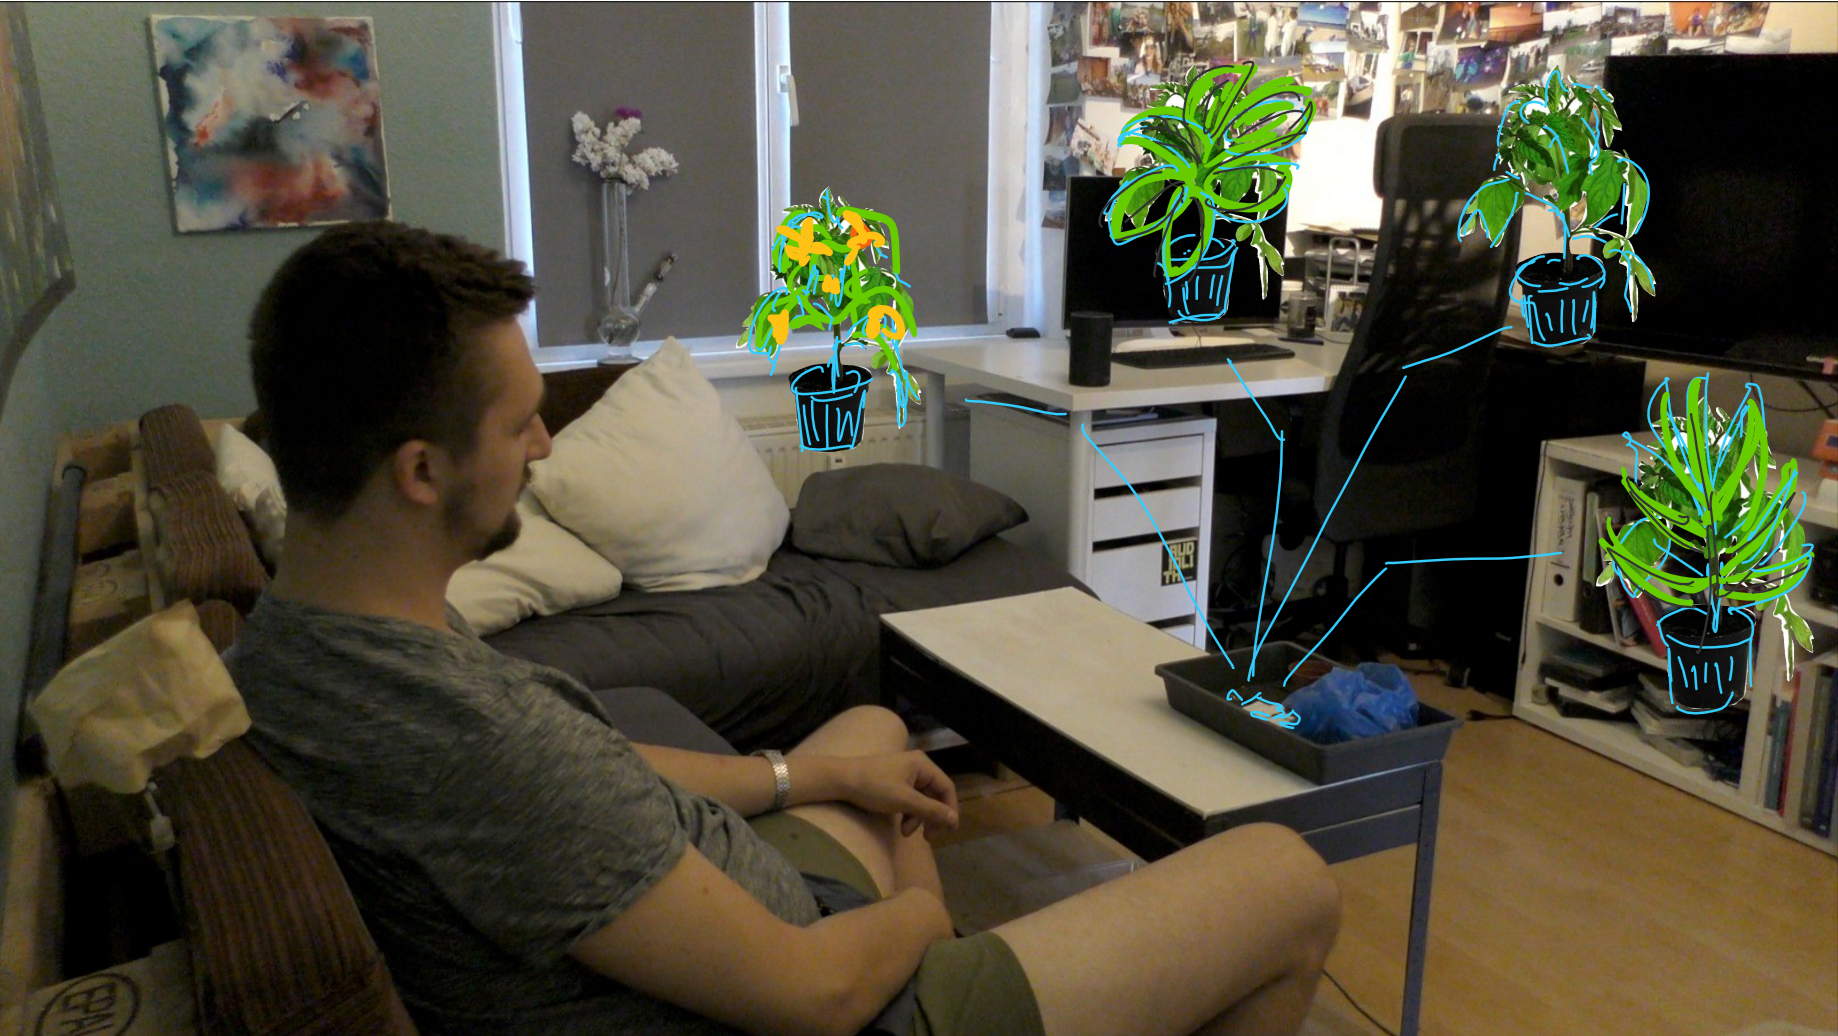
\includegraphics{img/UI/Pflanzenvisualisierung.png}
\caption{Pflanzenvisualisierung Variante 1}
\end{figure}

\begin{figure}
\centering
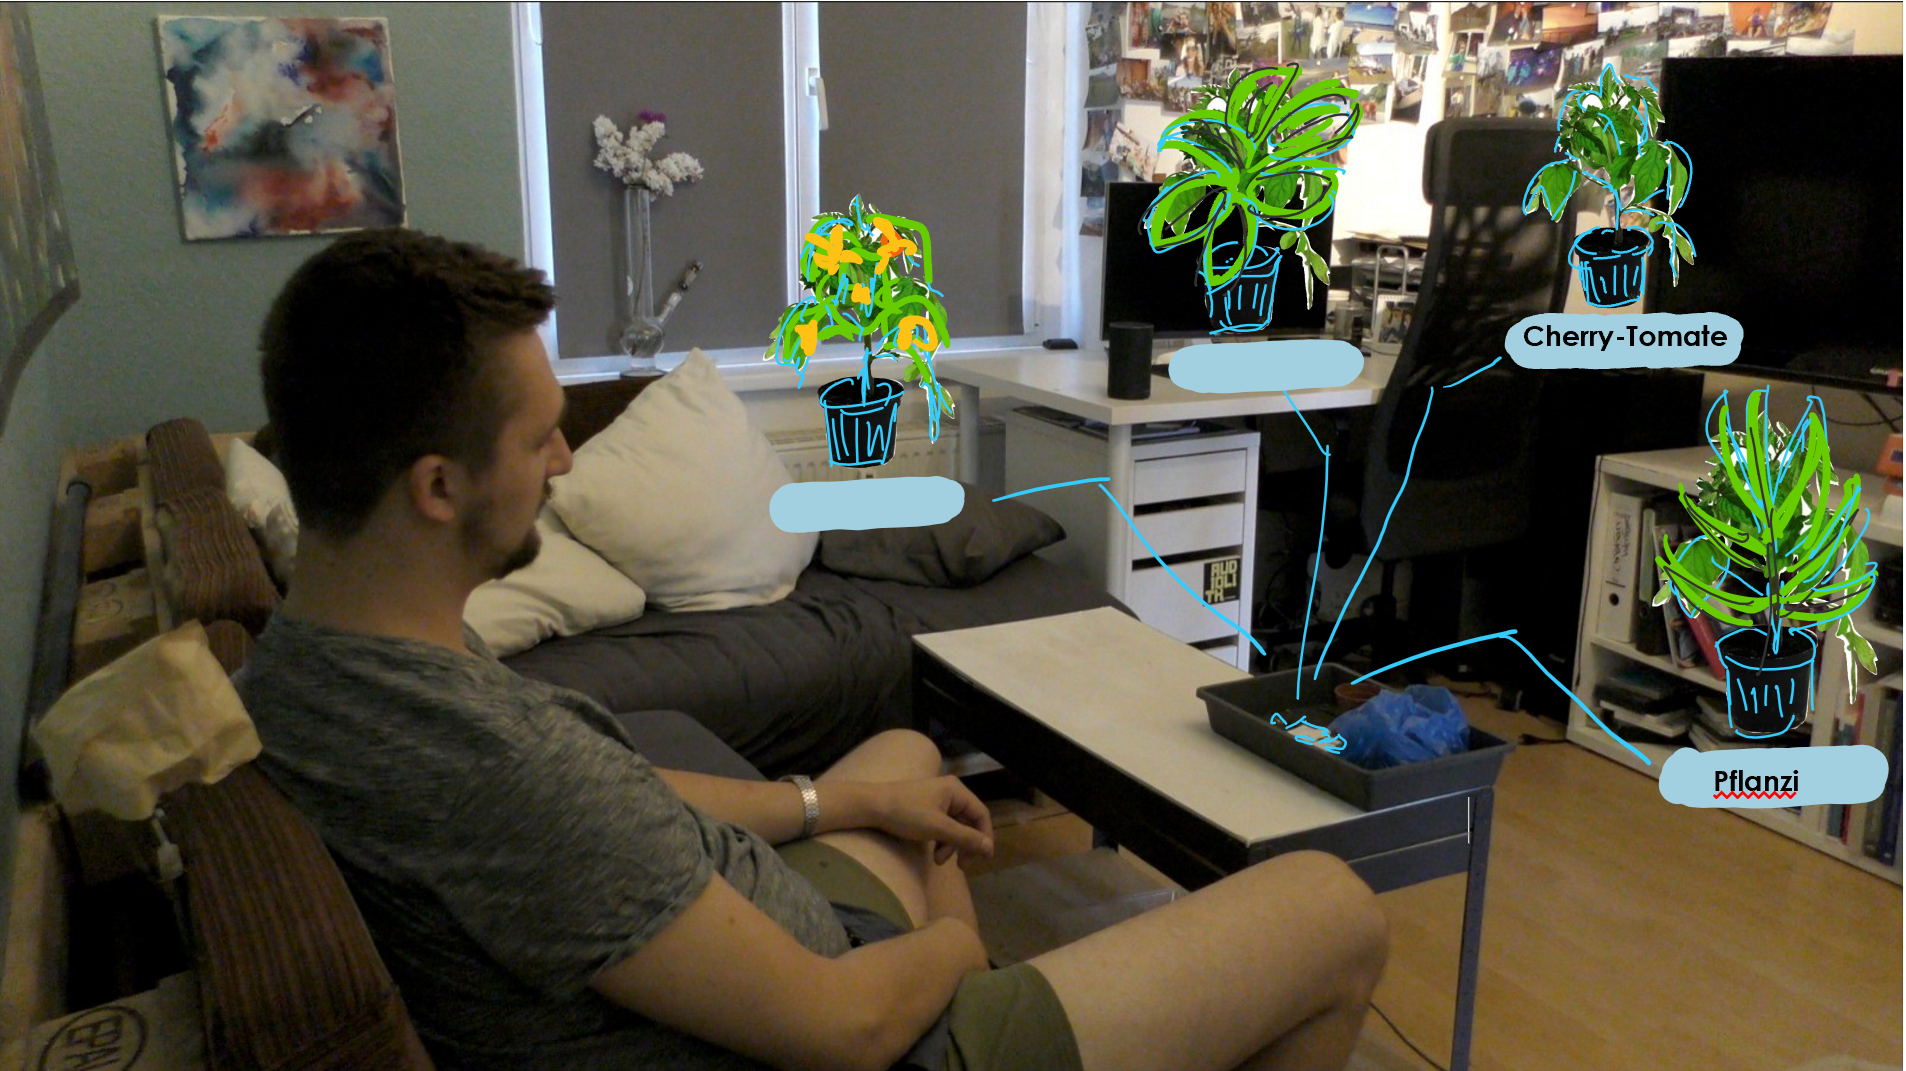
\includegraphics{img/UI/Pflanzenvisualisierung_mitNamen.png}
\caption{Pflanzenvisualisierung Variante 2}
\end{figure}

\begin{itemize}
\tightlist
\item
  Gestenerkennung → ``Greifen'' der Pflanzen, um mehr Informationen zu
  erhalten
\end{itemize}

\begin{figure}
\centering
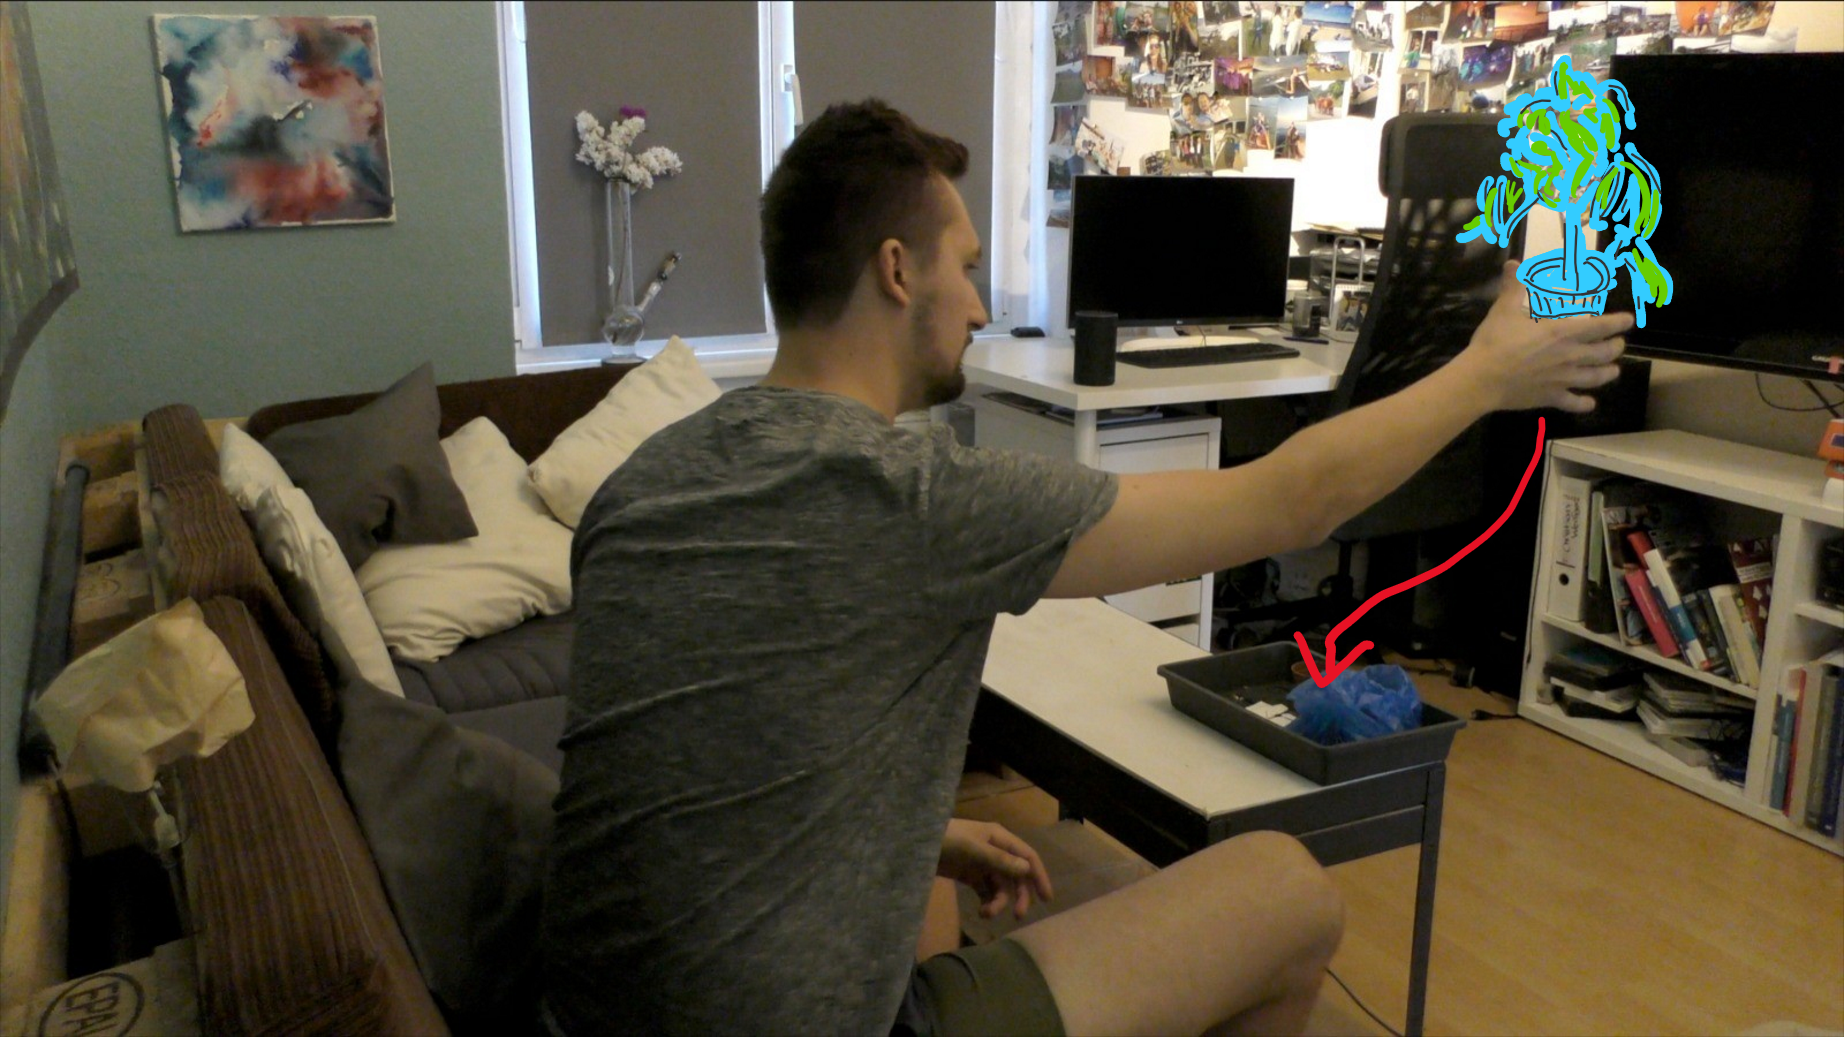
\includegraphics{img/UI/Greifen.png}
\caption{Gestenerkennung - Greifen}
\end{figure}

\begin{itemize}
\tightlist
\item
  Anzeige weiterer Informationen über die Pflanzen
\end{itemize}

\begin{figure}
\centering
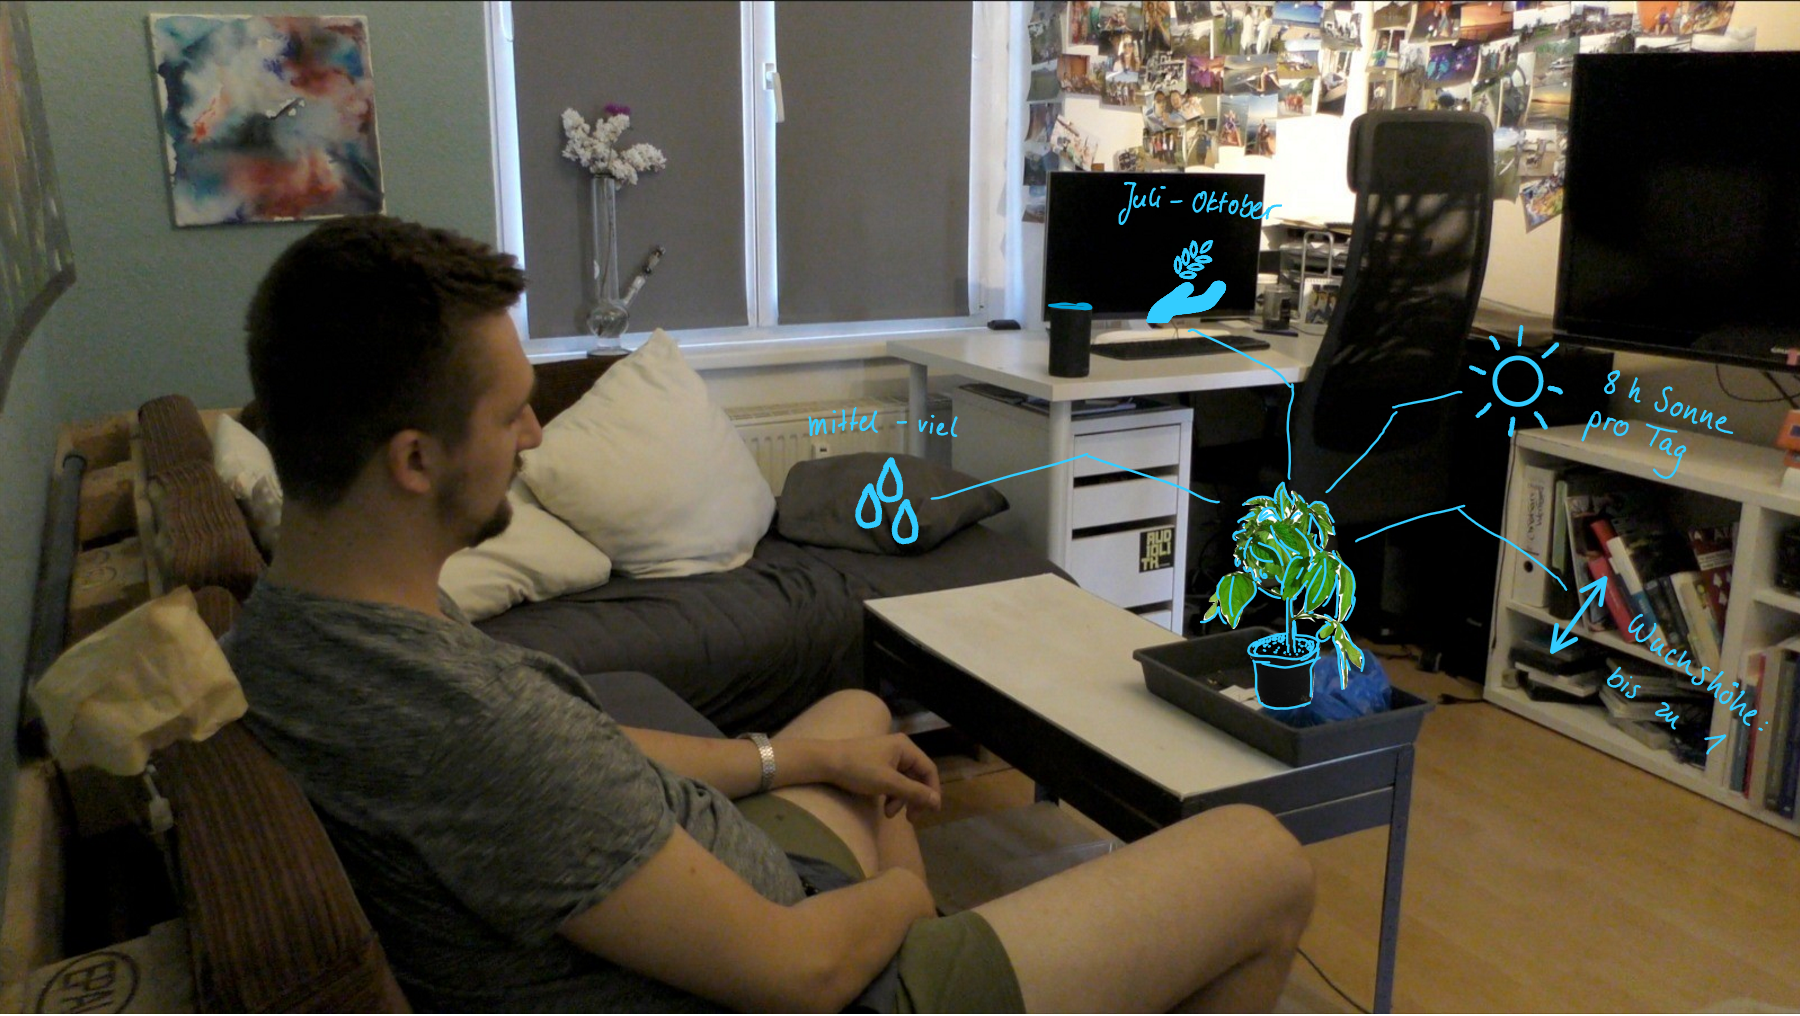
\includegraphics{img/UI/Steckbriefanzeige.png}
\caption{Steckbrief Variante 1}
\end{figure}

\begin{figure}
\centering
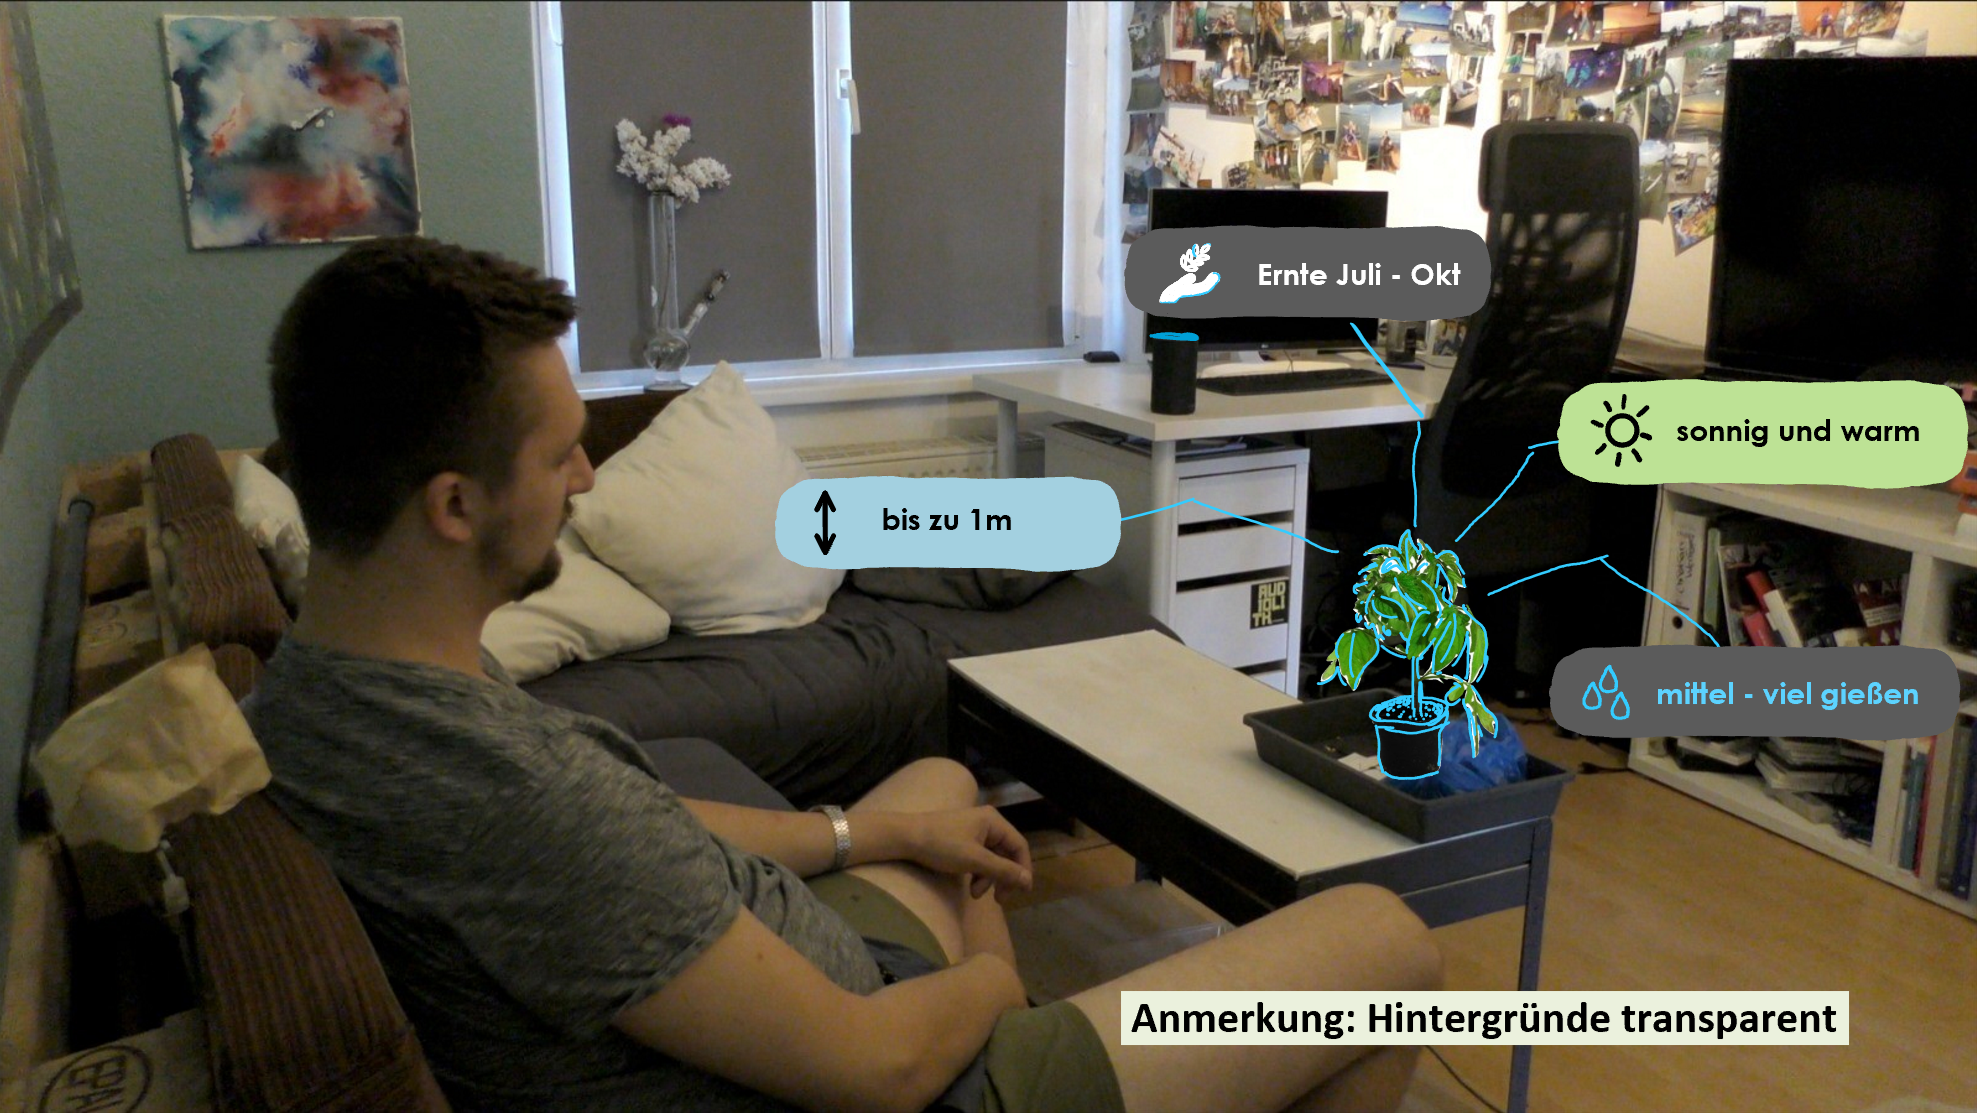
\includegraphics{img/UI/Steckbriefanzeige_verschVarianten.png}
\caption{Steckbrief Variante 2}
\end{figure}

\begin{itemize}
\tightlist
\item
  Analyse des Raumes und Erkennen eines guten Standortes für den
  Anzuchtkasten
\end{itemize}

\begin{figure}
\centering
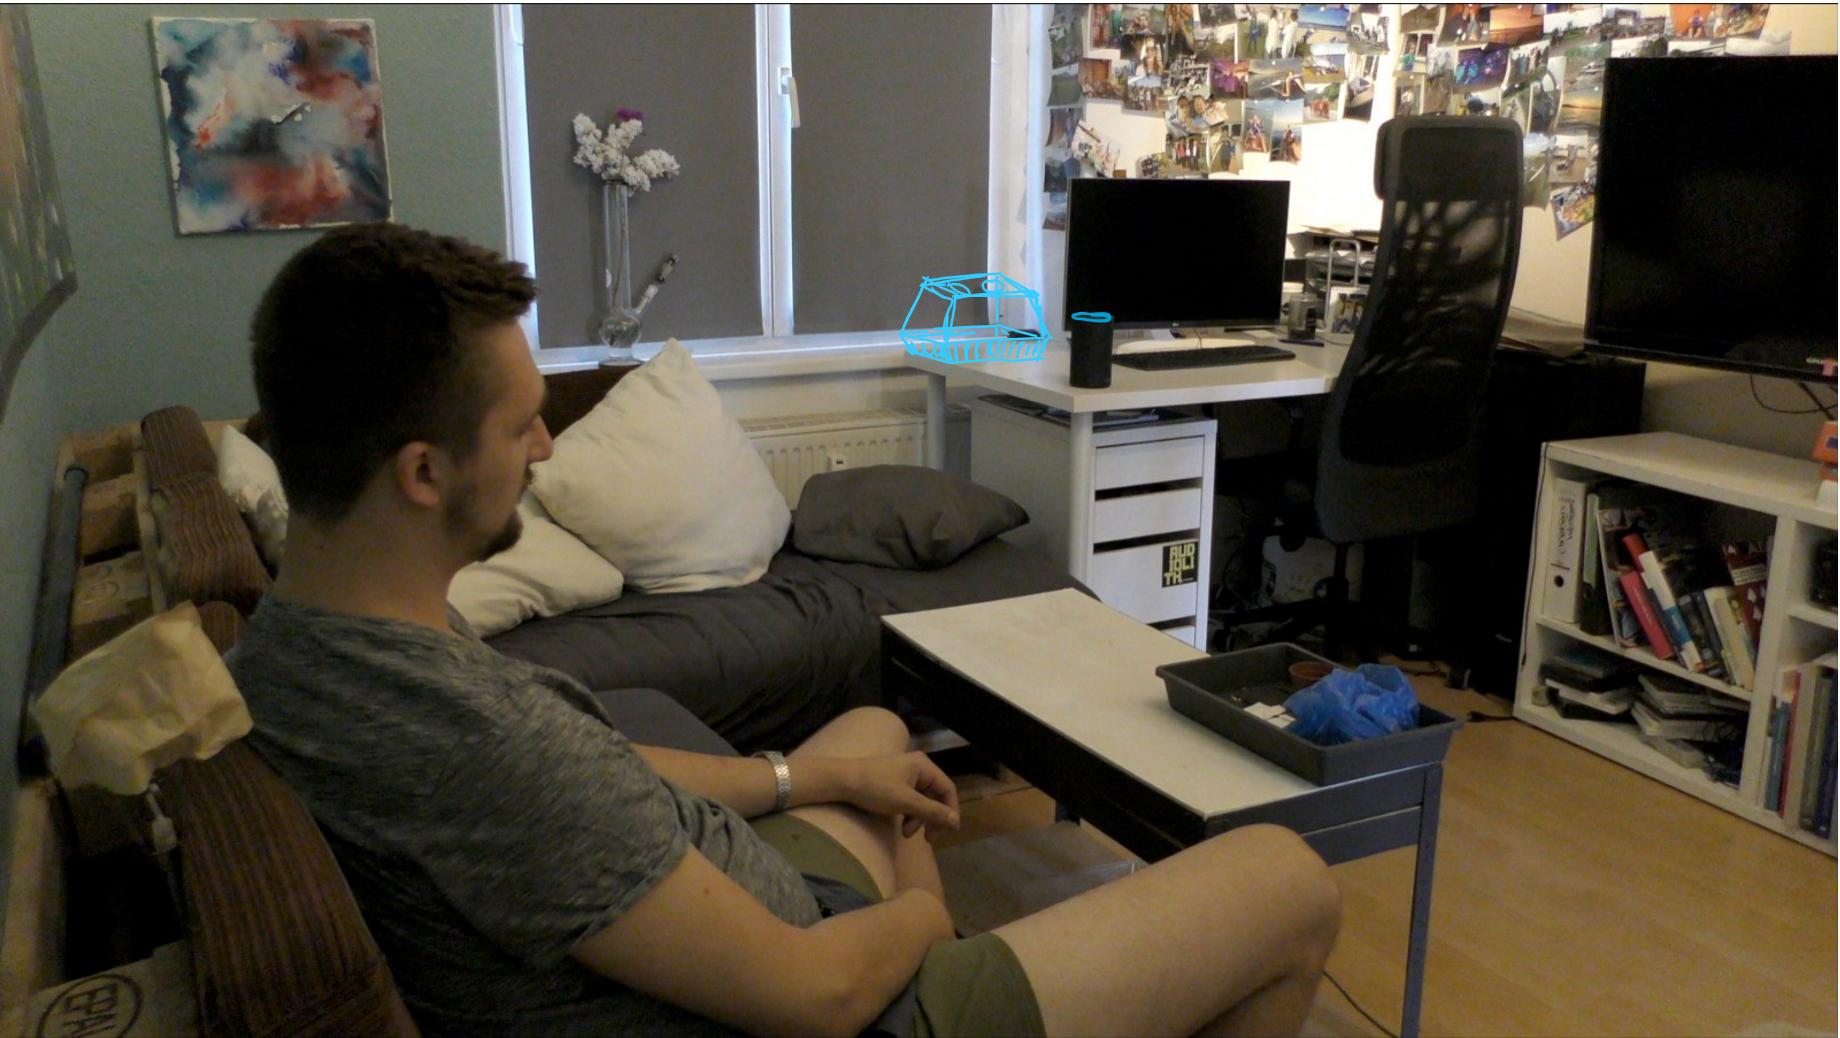
\includegraphics{img/UI/Raumscan4.png}
\caption{UI Raumscan 4}
\end{figure}

\begin{itemize}
\tightlist
\item
  Gestenerkennung → Unsicherheit Christians wird erkannt und Hilfe
  angeboten
\end{itemize}

\hypertarget{szene-3}{%
\paragraph{Szene 3}\label{szene-3}}

\begin{itemize}
\tightlist
\item
  Visualisierung des personifizierten Helfers → PLANT-E
\item
  Führen durch einen Ablauf (Eintopfen) mit Hilfe von PLANT-E
\item
  dabei wird der Fortschritt vom System erkannt und PLANT-E gibt dazu
  entsprechendes Feedback
\item
  Gießanzeige → zusätzliche Visualisierung zur Unterstützung, die
  unabhängig von PLANT-E ist
\end{itemize}

\hypertarget{szene-4}{%
\paragraph{Szene 4}\label{szene-4}}

\begin{itemize}
\tightlist
\item
  Erinnerungsfunktion → in dem Fall zum Umtopfen
\item
  Analyse der benötigten Utensilien und Angebot, dieselbigen zu
  bestellen
\item
  Fingerabdruck-Scanner zur Autorisierung der Bestellung
\end{itemize}

\begin{figure}
\centering
\includegraphics{img/UI/Badansicht.jpg}
\caption{Fingerabdruck-Scan}
\end{figure}

\hypertarget{szene-5}{%
\paragraph{Szene 5}\label{szene-5}}

\begin{itemize}
\tightlist
\item
  Führen durch einen Ablauf (Umtopfen) → wird nur in Grundzügen gezeigt,
  da das bereits vorgekommen ist
\item
  Sharing-Funktion → Fotografieren und Teilen mit den Freunden
\end{itemize}

\hypertarget{szene-6}{%
\paragraph{Szene 6}\label{szene-6}}

\begin{itemize}
\tightlist
\item
  Analyse des Pflanzenzustands (Reifegrad der Früchte) → Feedback und
  Handlungsempfehlung wird mit Hilfe von PLANT-E dem Nutzer mitgeteilt
\item
  Beetplanung → wird angedeutet mit den vielen neuen Töpfen auf dem
  Balkon

  \begin{itemize}
  \tightlist
  \item
    \emph{Anmerkung}: konnte aus Platzmangelgründen am Drehort nicht
    umgesetzt werden
  \end{itemize}
\item
  Sharing-Funktion → Funktion wird wieder aufgegriffen für die
  Endansicht
\item
  zeigt den Einsatz der App in verschiedenen Garten-, Beetgrößen und
  Szenarien
\item
  im Endeffekt nicht direkt dargestellt ist die mögliche Erweiterung auf
  automatisierte Versorgungssysteme (z.B. Bewässerung), durch die
  Karten-Endansicht wird aber angedeutet, dass es im Allgemeinen noch
  weitere Nutzungsmöglichkeiten gibt
\end{itemize}

\hypertarget{storyboard-und-drehplan}{%
\subsubsection{Storyboard und Drehplan}\label{storyboard-und-drehplan}}

Mit unseren Erfahrungen aus vorherigen Videoprojekten war klar, dass
eine gute Vorbereitung beim Dreh selber viele Unklarheiten und damit
Zeit ersparen. Verschiedene Anweisungen für den Dreh wurden bereits bei
der Erstellung des Drehbuches notiert, zum Schluss aber getrennt in
einem genauen Ablaufplan für den Dreh zusammengetragen. Dieser befindet
sich im \protect\hyperlink{anhang}{Anhang}.

Ebenso wichtig ist es gewesen, vor allem aus platz- und lichttechnischen
Gründen, vorausgehende Aufnahmetests am Drehort zu machen und daraufhin
die Erstellung eines Storyboards durchzuführen. Auch dieses befindet
sich im \protect\hyperlink{anhang}{Anhang}.

In einer weiteren Version des Drehbuchs\footnote{vgl. Link:
  \url{https://drive.google.com/drive/folders/1toOwAzorJRI8cY0EzBIM56n-LDfFUXsK}}
sind Verweise der verschiedenen Kameraeinstellungen in Bezug auf die
chronologische Handlung sowie auf gekennzeichnete Abschnitte des
Drehplans zu finden. Diese Verweise sind für den späteren Schnitt nötig
gewesen aufgrund der Tatsache, dass in manchen Szenen mehr
Kameraeinstellungen als zur Verfügung stehende Kameras geplant gewesen
sind.

\hypertarget{der-dreh}{%
\subsection{Der Dreh}\label{der-dreh}}

Der Drehtag war der 21.05.2020. Nach gründlich getroffenen
Vorbereitungen waren bereits nach ca. 6 Stunden alle Szenen aufgenommen
und der Dreh damit abgeschlossen.

\textbf{Akteure am Drehtag mit Funktion:}

\begin{itemize}
\tightlist
\item
  Christian Weniger: Hauptdarsteller in der Rolle des Christians
\item
  Hannes Dröse: Tonaufnahme / Sprecher für die Rollen von PLANT-E und
  Alexa
\item
  Robert Ackermann: Motion / UI Vision
\item
  Dennis Krischal: Kamera / Storyboard
\item
  Livia Schumm: Setdesign / Drehplan
\end{itemize}

\hypertarget{nachbearbeitung-des-videomaterials}{%
\subsection{Nachbearbeitung des
Videomaterials}\label{nachbearbeitung-des-videomaterials}}

\hypertarget{schnitt-und-ton}{%
\subsubsection{Schnitt und Ton}\label{schnitt-und-ton}}

Der hauptsächliche Zeitaufwand dabei ist definitiv in das Sortieren und
Zusammenfügen von Bild- und Tonaufnahmen geflossen, sprich den
Rohschnitt. Für die Stimmen von PLANT-E und Alexa wurde der Ton
gesondert aufgenommen, nachträglich mit Effekten bearbeitet und
anschließend dem Video hinzugefügt. Zur Audio-Bearbeitung ist
\textbf{Logic Pro X }verwendet worden.

Verwendet wurde das Schnittprogramm \textbf{Final Cut Pro}. Weitere
Arbeitsschritte sind gewesen:

\begin{itemize}
\tightlist
\item
  Anpassung der Belichtung (die Lichtverhältnisse am Drehort waren
  suboptimal, was sich in der Qualität der Bildaufnahmen zeigte)
\item
  das Erstellen einer Fotosequenz
\item
  den Feinschnitt mit Unterlegung von Musik
\item
  Zoom- und Übergangs-Effekte für die Schlusssequenz in der
  Kartenansicht
\item
  Erstellen des Abspanns mit Credits und Quellen
\end{itemize}

\textbf{Verwendete Musik:}

\begin{itemize}
\tightlist
\item
  Gianmara Testa - Gli Amanti di Roma
\item
  Adana Twins - Nobis
\end{itemize}

\textbf{Verwendete Schrift:} Amatic SC

Das Zwischenergebnis des Videos ohne animierte Komponenten findet sich
unter dem Link
\url{https://drive.google.com/drive/folders/1iqPfL00Kh-QehQd0OGzR-3Inb1JzLeHX}.

\hypertarget{animation}{%
\subsubsection{Animation}\label{animation}}

Die Animation von PLANT-E und den benötigten 3D-Modellen ist mithilfe
von Blender geschehen. Die Relation zum Realfilmanteil ist über dessen
Einfügen als Hintergrundebene geschaffen worden. Anschließend sind die
fertigen Animationen einzeln als png-Sequenzen exportiert worden.
Folgende Modelle, Animationen und Grafiken sind entstanden:\footnote{Alle
  zu finden im Google Drive Ordner ``Blender Export''
  \url{https://drive.google.com/drive/folders/1iVMQ3jvUBsfBQHznfuJ_IGur_D44yWXO}}

\textbf{PLANT-E}

\begin{itemize}
\tightlist
\item
  aufwendigstes Modell, darum ist sich hier einer Vorlage aus dem
  Videospiel ``Little Big Planet'' bedient worden\footnote{Link zur
    Quelle:
    \url{https://www.models-resource.com/playstation_3/littlebigplanet/model/7122/}}
\item
  dem Modell sind Haare hinzugefügt und ein Skelett verpasst worden
\item
  Gestik und Mimik sind animiert und an den Realfilm angepasst worden
\end{itemize}

\textbf{Pflanzenmodelle}

\begin{itemize}
\tightlist
\item
  ebenfalls Nutzung fertiger Modelle\footnote{Quelle: Sketchfab -
    Zvanstone, Link: \url{https://sketchfab.com/zvanstone}}
\item
  Animation der Bewegungen
\end{itemize}

\textbf{Objekte, Icons und Symbole}

\begin{itemize}
\tightlist
\item
  Modellierung Gießanzeige, Animierung des Füllstandes
\item
  Modellierung der benötigten Bestell-Objekte (Blumentopf, Sack
  Blumenerde, Sack Dünger)
\item
  Modellierung Fingerabdruck, Animation Farbverlauf
\end{itemize}

\textbf{Texteinblendungen}

Für den Bestellvorgang sind sowohl eine Version mit, als auch eine
Version ohne Schrift erstellt worden. Texteinblendungen haben sich
später allerdings in Hinblick auf ein einheitliches Bild mehr in After
Effects angeboten.

\hypertarget{zusammenfuxfcgen-der-komponenten}{%
\subsubsection{Zusammenfügen der
Komponenten}\label{zusammenfuxfcgen-der-komponenten}}

Zu guter Letzt sind alle erstellten Film-Komponenten zusammengefügt und
der Feinschliff für ein rundes Gesamtbild erschaffen worden. Hierfür ist
als Tool \textbf{Adobe After Effects} zum Einsatz gekommen.

Die Arbeitsschritte sind gewesen:

\begin{itemize}
\tightlist
\item
  das Einfügen und Anpassen der Animationen in den Realfilmanteil
\item
  holografische Effekte erschaffen
\item
  Optik anpassen, übergreifendes Design schaffen (angelehnt an
  UI-Design)
\item
  Kreation des Raumscan-Effektes
\item
  Texte und Textfelder erstellen, platzieren, animieren, Design und
  Effekte anpassen
\item
  holografische Nachricht der Schwester sowie Kamera-Schnappschuss von
  Christian erstellen
\item
  Verdeckungen (davon reichlich)
\item
  Stecknadeln und Garten-Posts auf Kartenansicht setzen, Motion Tracking
  mithilfe von Markern
\item
  Einbauen von Details → Feinschliff
\end{itemize}

\textbf{Verwendete Schrift:} Vox Round Semibold

\hypertarget{fazit-zum-ergebnis-video}{%
\subsection{Fazit zum Ergebnis-Video}\label{fazit-zum-ergebnis-video}}

\hypertarget{aufgetretene-herausforderungen-und-der-umgang-damit}{%
\subsubsection{Aufgetretene Herausforderungen und der Umgang
damit}\label{aufgetretene-herausforderungen-und-der-umgang-damit}}

\textbf{Die Herausforderung der Prioritätenlegung:}

Bei der Entwicklung des Drehbuches hat sich vor allem die Frage
gestellt, inwieweit sich in einem kurzen Zeitrahmen eine schöne
Geschichte erzählen lässt, bei der eine Produktvision mit ihren Features
deutlich vermittelt wird. Gerade der Grad an Interaktion zwischen Mensch
und Maschine hat immer wieder im Fokus gestanden und hat zu wiederholt
nötigen Absprachen und mehrmaligen Überarbeitungen des Drehbuches
geführt.\footnote{vgl. Asana-Protokolle KW19
  (\url{https://app.asana.com/0/1172859492234369/1174005793106255}) bis
  KW21 (\url{https://app.asana.com/0/1172859492234369/1176239239126747})}

\textbf{Nachträgliche Visualisierung:}

Die Interaktionsgestaltung ist zwar bereits vor dem Dreh bei der
Erstellung von Storyboard und Drehplan kommuniziert worden, visuell
skizziert allerdings erst hinterher. Teilweise ist dann mit
Bildausschnitten gearbeitet worden, die man noch optimieren hätte
können.

\textbf{Auch gute Vorbereitung schafft neue Herausforderungen:}

Dank des Storyboards und des Drehplans ist ein reibungsloser Dreh
möglich gewesen. Allerdings sind die Kameras durchgängig am Laufen
gewesen. Der Drehort ist sehr eng, wodurch die Kameras schlecht
zugänglich gewesen sind. Im Schnitt ist später dadurch ein enormer
Mehraufwand entstanden, da alleine für den Rohschnitt große Mengen an
Videomaterial gesichtet und aussortiert werden mussten.

\textbf{Koordination der Arbeitsschritte in der Videonachbearbeitung:}

Aus technischen Gründen ist die Reihenfolge von Schnitt, Animation und
After Effects größtenteils nur nacheinander möglich gewesen. Es ist also
nur teilweise parallel am Video gearbeitet worden und so sind immer
wieder unterschiedliche Teile des Teams ausgebremst worden. Dadurch ist
der Zeitrahmen sehr schwierig abzuschätzen gewesen. Gerade der letzte
Schritt, das Zusammenfügen von Komponenten aus Realfilm und Animation
ist von der Fertigstellung dieser vorausgehenden Komponenten abhängig
gewesen und im Umfang unterschätzt worden.

In diesem Projektabschnitt sind Absprachen und Koordination also eine
besondere Herausforderung gewesen, sind aber dank regelmäßiger Meetings
sowie der sorgfältigen Protokollierung von Entscheidungsprozessen in
Asana gut gemeistert worden.

\textbf{Auslastung beim Arbeiten mit Grafik-Programmen:}

Ein immer wiederkehrendes Problem bei Projekten in der Mediengestaltung
ist die Größe der Datenmengen und die Auslastung von Geräten. Hilfreich
ist dann beispielsweise die Erkenntnis gewesen, dass After Effects erst
dann eine arbeitsfähige Performance zeigt, wenn der lokale Speicher mehr
als 14GB unbelegt zur Verfügung hat. So sind die größten anfänglichen
Schwierigkeiten mit einfachem Aufräumen von Speicherplatz gelöst worden.

\hypertarget{ausblick-und-auswertung}{%
\subsubsection{Ausblick und Auswertung}\label{ausblick-und-auswertung}}

Folgende Aspekte am Video sind im Endeffekt ausbaufähig geblieben:

\begin{itemize}
\tightlist
\item
  in größerem Zeitrahmen Darstellung weiterer (evtl. aller) Features
\item
  Genauigkeit bei den Verdeckungen
\item
  weitere Soundeffekte (z.B. beim Erscheinen und Verschwinden von
  PLANT-E)
\item
  in der Schlusssequenz des Videos ist außerdem die Schnitt-Taktung auf
  die Musik noch optimierbar
\end{itemize}

Insgesamt befindet das Team das Ergebnis-Video jedoch als
zufriedenstellend. Wie bei den meisten gestalterischen Projekten sind
die anfänglichen Vorstellungen in der Praxis aufgrund damit verbundener
Zeitaufwände auf das Wesentliche beschränkt worden. Der Anspruch dabei
ist dennoch gewesen, zu einem insgesamt abgerundeten Ergebnis zu kommen,
das für den Betrachter sowohl ansprechend als auch verständlich ist.
Dies ist glücklicherweise gelungen.

\hypertarget{prototyp}{%
\section{Der Prototyp}\label{prototyp}}

\hypertarget{konzeption}{%
\subsection{Konzeption}\label{konzeption}}

\hypertarget{idee}{%
\subsubsection{Idee}\label{idee}}

Aus dem Visionsvideo soll nun ein Prototyp entwickelt werden, der einen
ersten Schritt in Richtung Realisierung der Vision darstellen soll.

Selbstverständlich sind Hologramm-Technologien, wie sie im Video gezeigt
werden, noch längst nicht umsetzbar. Allerdings gibt es heute schon
Möglichkeiten virtuelle Objekte in die reale Welt zu setzen und zwar in
Form von Augmented Reality.

Der Aspekt, dass die Anwendung auf so ziemlich jedem Gerät laufen soll,
lässt sich realisieren: Der Prototyp wird eine Web-Anwendung. Dadurch
geht allerdings auch ein Aspekt verloren: Man kann dem Nutzer keine
Erinnerungen/Notifications schicken, wenn er sich nicht auf der Webseite
befindet. Diese Einschränkung nimmt das Team für den Prototypen aber in
Kauf.

Das Erkennen von Pflanzen und ihrem Zustand anhand von Scans bzw.
Bildern ist zwar prinzipiell möglich, allerdings sind solche
Analysesysteme sehr aufwendig und brauchen sehr viele Testdaten, um
richtig funktionieren zu können. Das würde den Projektrahmen sprengen.
Daher wird der Prototyp nur mit einem Anzuchtkasten umgesetzt, in den
zusätzlich Sensoren eingebaut werden.

Zusammengefasst soll also eine AR-Anwendung im Webbrowser realisiert
werden, die mit einem Anzuchtkasten funktioniert. In den Anzuchtkasten
werden Sensoren eingebaut, die den Zustand im Kasten erfassen. Über
mobile Endgeräte erfolgt nun die Überlagerung von virtuellen Objekten in
die reale Welt, gestützt durch die Messwerte der Sensoren.

\hypertarget{design}{%
\subsubsection{Design}\label{design}}

Das daraus abgeleitete Design findet sich in der Grafik wieder.
Alternativ befindet es sich ebenfalls im
\protect\hyperlink{anhang}{Anhang}.

\begin{figure}
\centering
\includegraphics{img/AblaufVisualisierung_kompr.jpg}
\caption{Grafik - Ablauf und Visualisierung}
\end{figure}

Die Messdaten der Sensoren werden unterschieden in
\textbf{übergreifende} und \textbf{spezifische} Messdaten.
Luftfeuchtigkeit, Belichtung und Temperatur gelten für alle Pflanzen im
Kasten gleich, darum werden sie auch in der Darstellung an den Kasten
angehängt und direkt im Startmenü angezeigt. Lediglich die
Bodenfeuchtigkeit gilt spezifisch für jeden Topf einzeln, der User muss
diesen Topf also zunächst im Startmenü auswählen, um sich dessen gesamte
Daten unter der Menüoption ``Standortdaten'' anzeigen zu lassen.

Außerdem unterschieden werden muss zwischen einem leeren und einem
bepflanzten Topf. Je nachdem wie diese Zustandseigenschaft des Topfes
belegt ist, ergeben sich bei der Auswahl dessen nämlich auch weitere zu
unterscheidende Menü- und Aktivitäts-Optionen. Diese lassen sich der
Ablauf-Grafik entnehmen.

Übergreifende Messdaten werden über dem Kasten als türkise Buttons
dargestellt. Durch Antippen wird zum jeweiligen Messwert ein Diagramm
angezeigt, welches den Verlauf über die letzten Tage visualisiert.

Umfangreichere Inhalte wie Informationen zu einer Pflanze oder auch die
Diagramme werden in einem weißen Popup dargestellt, welches sich auf den
Bildschirm legt und die AR-Szene überdeckt. Das Popup ist am Bildschirm
fest und nicht am Kasten. Er ist scrollbar und kann über ein X
geschlossen werden.

Wichtige Notifications, welche in der Grafik rot dargestellte Symbole
sind, erscheinen, falls ein nötiger Handlungsbedarf besteht (z.B. wenn
die Erde der Pflanze zu trocken ist), am jeweiligen Topf. Durch Antippen
sollen diese direkt zu einer entsprechenden Popup-Nachricht führen und
zu der erforderlichen Aktion im Menü navigieren.

Popup-Nachrichten sind immer unten zu sehen in Form von Sprechblasen,
die von PLANT-E ``gesprochen'' werden. Diese Popup-Nachrichten sollen
auch die Anweisungen z.B. für das Eintopfen darstellen. Dies soll die
Kommunikation von PLANT-E mit dem Nutzer visualisieren.

\hypertarget{architektur}{%
\subsection{Architektur}\label{architektur}}

Aus diesen Anforderungen ist eine Architektur entstanden, die aus drei
Kernkomponenten besteht:

\begin{itemize}
\tightlist
\item
  dem Sensorenhandling über einen Raspberry Pi,
\item
  der Datenverwaltung und Auslieferung der Webseite über einen
  Backend-Server und
\item
  die eigentliche Webseite, die von den Clients aufgerufen wird.
\end{itemize}

Zur Übersicht ist ebenfalls ein Diagramm erstellt worden, welches die
Komponenten und ihr Zusammenspiel verdeutlicht.

\begin{figure}
\centering
\includegraphics{img/architektur.png}
\caption{Grafik der Architektur}
\end{figure}

Die Sensordaten werden stetig gemessen und vom Raspberry Pi über
UDP-Pakete an das Backend gesendet. UDP ist ein verbindungsloses
Protokoll. Es werden lediglich Zieladresse und -port angegeben und schon
wird das Datenpaket versendet. Es findet keine Empfangsbestätigung
statt. Die Pakete sind immer kleine abgeschlossene Einheiten. Die Idee
ist, dass die Sensordaten in einem langen konstanten Datenstrom
ausgeliefert werden, egal ob jemand diese Daten entgegennimmt oder
nicht. Die Vorstellung eines Radiosenders ist ein geeigneter Vergleich.
Der Vorteil dieses Vorgehens ist, dass stetig und sehr schnell Daten zur
Verfügung stehen mit geringstem Overhead.

Der Backend-Server ist das Bindeglied für alle Komponenten. Er nimmt den
UDP-Datenstrom des Raspberry Pis entgegen und verarbeitet diese Daten.
Zum Einen werden sie für die Erfassung eines historischen Verlaufes
gespeichert. Zum Anderen können die Daten vom Frontend nun abgerufen
werden. Das Backend liefert immer die aktuellensten erhaltenen Daten
aus. Bricht der Datenstrom vom Raspberry Pi ab, sind immer noch die
zuletzt empfangenen Daten abrufbar.

Zusätzlich liefert das Backend auch die Frontend-Webseite mit allen
zugehörigen Dateien aus. Darüber hinaus stellt das Backend eine REST-API
zur Verfügung, die vom Frontend genutzt werden kann, um Daten abzurufen
und zu senden. Die Speicherung von zusätzlichen Daten, z.B. ob ein Topf
bepflanzt ist und wie lange schon, wird ebenfalls im Backend gespeichert
und verwaltet. Das Backend liefert auch einen Pflanzenkatalog mit den
unterstützen Pflanzenarten aus.

Das Frontend ist eine Webseite, die in jedem modernen Browser aufgerufen
werden kann. Da es sich um eine AR-Anwendung handelt, benötigt der
Client zwingend eine Kamera im Gerät. Die Anwendung ist nur in der Lage
Informationen rund um den Kasten anzuzeigen. Zur Erkennung des Kastens
ist dort ein Marker angebracht dazu -- später mehr.

\hypertarget{umsetzung}{%
\subsection{Umsetzung}\label{umsetzung}}

\hypertarget{raspberry-pi}{%
\subsubsection{Raspberry Pi}\label{raspberry-pi}}

Der Raspberry Pi soll mittels Sensoren verschiedene Daten zu dem
Anzuchtkasten messen und per UDP-Pakete an das Backend senden.

\hypertarget{datenformat}{%
\paragraph{Datenformat}\label{datenformat}}

Die gesendeten UDP-Pakete sollen alle Messdaten im JSON-Format
enthalten. Hier die Spezifikation der zu sendenden Daten:

\begin{verbatim}
{
  "timestamp": 1594639596, // unix timestamp
  "airHumidity": 42, // in Prozent, ganzzahlig
  "light": 123,      // in lux, ganzzahlig
  "temperature": 24, // in Grad, ganzzahlig
  "pots": [ // die Töpfe von links nach rechts
    {
      "soilHumidity": 73, // in Prozent, ganzzahlig
      // "size": 8,       // Höhe der Pflanze in cm
                      // ist nicht umgesetzt worden
    }
  ],
}
\end{verbatim}

Luftfeuchtigkeit, Helligkeit und Temperatur werden für den gesamten
Kasten erfasst. Die Bodenfeuchtigkeit wird für jeden Topf einzeln
gemessen und ausgeliefert. Da der Gruppe nur ein Sensor für die
Bodenfeuchtigkeit zur Verfügung gestellt worden ist, kann der Prototyp
nur einen Topf bedienen.

Die Analyse der Wuchshöhe ist im Verlaufe des Projektes ausgeklammert
worden, da keine geeignete Kamera zur Verfügung gestanden hat. Außerdem
ist die Analyse von Kamerabildern ein recht aufwendiges Verfahren, was
den Rahmen des Projektes gesprengt hätte.

\hypertarget{verwendete-sensoren}{%
\paragraph{Verwendete Sensoren}\label{verwendete-sensoren}}

Zum Verarbeiten der Sensordaten wird ein Raspberry Pi 4 benutzt, da
dieser der Projekt-Gruppe bereits zur Verfügung gestanden hat. Für die
Sensoren ist daher die Auswahl etwas begrenzt gewesen.

\begin{itemize}
\tightlist
\item
  Lichtmessung: \emph{Lichtsensor „BH1750``}

  \begin{itemize}
  \tightlist
  \item
    wandelt bereits auf der Platine die Analogsignale in Digitalsignale
  \end{itemize}
\item
  Messung von Temperatur und Luftfeuchtigkeit: \emph{Sensor „DHT22``}

  \begin{itemize}
  \tightlist
  \item
    wandelt ebenso bereits die Signale, sodass diese ohne zusätzliche
    Bauteile vom Raspberry Pi gelesen werden können
  \end{itemize}
\item
  Messung der Bodenfeuchtigkeit: \emph{„Capacitive Stil Moisture Sensor
  v2.0``}

  \begin{itemize}
  \tightlist
  \item
    wurde von Hardwareexperten der FH empfohlen
  \item
    liefert unter den Feuchtigkeitssensoren wohl die präzisesten Daten
  \end{itemize}
\item
  Signalverarbeitung des Feuchtigkeitssensors: \emph{Analog-Digital
  Wandler „MCP3008``}

  \begin{itemize}
  \tightlist
  \item
    wurde ebenso gewählt aufgrund der Empfehlung führender
    Hardwareexperten der FH
  \end{itemize}
\end{itemize}

Um diese Sensoren auf dem Raspberry Pi nutzen zu können sind externe
Bibliotheken nötig gewesen. Hierbei handelt es sich um:
Adafruit\_ADSx15\footnote{Link:
  \url{https://github.com/adafruit/Adafruit_Python_ADS1x15}},
Adafruit\_DHT\footnote{Link:
  \url{https://github.com/adafruit/Adafruit_Python_DHT}} und
smbus\footnote{Link:
  \url{http://wiki.erazor-zone.de/wiki:linux:python:smbus:doc}}.

\textbf{Anmerkung zur Abgrenzung zwischen dem Gruppenprojekt ``Grüni''
und dem IT-Praxisprojekt von Dennis Krischal:}\\
Die Projekte überschneiden sich in genau einem Punkt, da es sich
angeboten hat für beide die gleiche Hardware zum Auslesen der Sensoren
zu benutzen.

\hypertarget{schaltplan}{%
\paragraph{Schaltplan}\label{schaltplan}}

\begin{figure}
\centering
\includegraphics{img/schaltplan.png}
\caption{Schaltplan der Sensoren mit dem Raspberry Pi}
\end{figure}

\hypertarget{skript}{%
\paragraph{Skript}\label{skript}}

Die Anwendung auf dem Raspberry Pi ist als Python-Skript erstellt
worden. Es liest die Sensordaten und versendet sie als UDP-Paket an den
Server.

Es gibt einen Mock-Modus in dem das Skript keine Sensordaten, sondern
Zufallswerte generiert und ausgibt. Das Skript kann dadurch auch auf
einem beliebigen Gerät gestartet werden, liefert dann aber natürlich nur
die Zufallswerte.

\hypertarget{backend}{%
\subsubsection{Backend}\label{backend}}

Das Backend ist ein Node.js-Server, der in TypeScript implementiert
worden ist. Er empfängt zum einen die UDP-Pakete vom Raspberry Pi über
einen entsprechenden Socket. Zum Anderen stellt er einen Express.js
Server zur Verfügung, der sowohl das Frontend inklusive aller benötigten
Dateien ausliefert als auch eine REST-API für das Frontend zur Verfügung
stellt.

Es speichert die Daten vom Raspberry Pi in regelmäßigen Abständen in
einer Historie und speichert auch Daten, die vom Frontend kommen. Zum
Beispiel in welchem Topf sich welche Pflanze befindet und wie lange die
dort schon eingetopft ist usw.

Außerdem liegt ein Katalog mit den unterstützten Pflanzenarten im
Backend vor. Dieser wird verwendet, um die Pflanzendaten anzureichern.

Die Daten werden in JSON-Dateien gespeichert, die beim Start des Servers
geladen werden. Ändern sich die Daten, so werden die Änderungen auch in
die JSON-Dateien geschrieben. Die Verwendung von einem
Datenbanken-System ist für den Prototypen zu aufwendig gewesen.

\hypertarget{frontend}{%
\subsubsection{Frontend}\label{frontend}}

Das Frontend besteht aus einer Webseite, die von der Funktion her eine
SPA (Single-Page-Application) ist. Zum Einsatz kommt das Webframework
\textbf{Vue.js} sowie die Technologien \textbf{AFrame} und
\textbf{AR.js}.

\textbf{Vue.js}\footnote{Link: \url{https://vuejs.org}} ist ein
schlankes Frontend-Framework, welches mit recht simplen HTML-Attributen,
einem Komponenten- und Vorlagensystem das erstellen von interaktiven
Webseiten vereinfacht. Es kann einfach auf die HTML-Struktur
draufgesetzt werden und ist recht leichtgewichtig.

\textbf{AFrame}\footnote{Link: \url{https://aframe.io}} ist ein Wrapper
für Three.js, mittels dem 3D-Modelle in eine Szene gesetzt und gerendert
werden können. AFrame stellt dabei HTML-Tags zur Verfügung, die
3D-Elemente repräsentieren und entsprechend gerendert werden. Der
Mechanismus erfolgt so, dass ein
\texttt{\textless{}a-scene\textgreater{}}-Tag im HTML-Markup gesetzt
werden muss. Diese \texttt{\textless{}a-scene\textgreater{}} wird dann
in ein HTML-Canvas-Element umgewandelt und die 3D-Elemente
(\texttt{\textless{}a-entity\textgreater{}}) innerhalb der
\texttt{\textless{}a-scene\textgreater{}} werden in die Szene gesetzt
und auf den Canvas gemalt. Mit diesem System lassen sich VR-Anwendungen
im Webbrowser darstellen.

\textbf{AR.js}\footnote{Link:
  \url{https://ar-js-org.github.io/AR.js-Docs/}} ist nun eine
Erweiterung für AFrame. Der zugrundeliegende Mechanismus bleibt gleich,
allerdings wird der Hintergrund des Canvas mit dem Bild der
geräteinternen Kamera gefüllt. Zusätzlich kann ein sog. Marker definiert
werden (siehe Bild). Der Marker wird vom Kamerabild erkannt und dient
als Referenzpunkt. Die Position des Markers markiert den Ursprungspunkt
der Szene (Punkt 0,0,0). Die Breite des Markers gibt die Breite von
einer Einheit in AR.js an. Nun können 3D-Elemente relativ zum Marker
platziert werden.

\begin{figure}
\centering
\includegraphics{img/hiro.png}
\caption{Bild des Hiro-Markers von AR.js}
\end{figure}

AR.js funktioniert so, dass die Elemente nur zu sehen sind, wenn auch
der Marker zu sehen ist, zu dem die Elemente ja relativ liegen. Er dient
als Referenz- und Ankerpunkt der Szene. Der Einfachheit halber ist der
Standard-Marker von AR.js verwendet worden.

\hypertarget{ergebnisse-und-herausforderungen}{%
\subsection{Ergebnisse und
Herausforderungen}\label{ergebnisse-und-herausforderungen}}

Die Umsetzung des Raspberry Pi, der Sensoren und des Backends hat sehr
gut funktioniert. Die Daten werden richtig ausgeliefert, im Backend
gespeichert und ausgegeben. Lediglich die Geschwindigkeit der Sensoren
ist nicht optimal. Diese brauchen im Schnitt etwas unter einer Sekunde,
um die Messdaten zu erheben und zu versenden. Dies ist für sehr
interaktive Use-Cases wie zum Beispiel der Gießanzeige zwar unpraktisch,
für den Prototypen ist es aber ausreichend. Hier können in Zukunft
Optimierungen vorgenommen werden, etwa mit besserer Hardware.

Bezüglich des Backends fehlen natürlich reale, über einen längeren
Zeitraum erhobene Daten. Wären diese vorhanden, könnten sich noch neue
Erkenntnisse gewinnen und zum Beispiel eine sehr umfangreiche Historie
mit vielen Optionen und Ansichten erzeugen lassen. Für einen Protoypen
sind die vorhandenen Daten aber ausreichend.

Sehr ernüchternd ist hingegen das Frontend ausgefallen. Die anfängliche
Euphorie über die AR-Technik im Browser ist sehr schnell verflogen, weil
sich sehr bald gravierende Schwierigkeiten ergeben haben. Der
Projektfortschritt ist dadurch so stark behindert worden, dass nur ein
Bruchteil der geplanten Funktionalität überhaupt umgesetzt werden
konnte.

Ein großes Problem, welches immernoch nicht abschließend gelöst werden
konnte, ist das Anklicken von Elementen in AR.js. Es hat sehr lange
gedauert, bis es überhaupt möglich gewesen ist, auf Klicks zu reagieren.
Das hängt damit zusammen, dass Klicks in der Szene über einen Raycaster
umgesetzt werden. Dieser Raycaster ist in der Standard-Konfiguration zu
langsam. Da im AR-Modus die Szene ständig verschoben wird, aufgrund des
wackelnden Markers durch die wackelige Hand des Nutzers, muss der
Raycaster sehr schnell immer wieder nach Kollisionen checken, ansonsten
werden niemals irgendwelche Klicks erkannt. Diese Erkenntnis zu gewinnen
und das Problem zu lösen, hat alleine 2 Wochen in Anspruch genommen.

Damit nicht genug funktionieren Klicks im AR-Modus nur in der Mitte des
Bildschirms einigermaßen zuverlässig. Weiter am Rand funktionieren sie
so gut wie gar nicht. Die genaue Ursache ist bis heute nicht geklärt
worden. Durch das Wackeln werden zusätzlich manchmal Element angeklickt,
die man gar nicht klicken wollte. Insgesamt ist das Interagieren mit der
AR-Anwendung sehr mühselig und ist alles andere als intuitiv und
ausgereift.

Auch die Erkennung des Markers in AR.js funktioniert nur unter guten
Lichtverhältnissen und freie Sicht der Kamera auf den Marker. Wird der
Marker verloren, so verschwinden einfach alle 3D-Elemente. Dies stellt
keine schöne User Experience dar und ist gerade für die Entwicklung sehr
anstrengend.

Deswegen ist während der Entwicklung der AR-Modus meistens ausgeschaltet
gewesen. Die App wurde hauptsächlich im VR-Modus entwickelt, da hier
nichts wackelt und die Entwickler besser testen können, was sie
eigentlich tun. Daher funktioniert die Anwendung im VR-Modus recht gut,
im AR-Modus eher weniger.

Auch im Design sind die Möglichkeiten von AFrame und AR.js sehr
beschränkt. So ist es nicht möglich zum Beispiel die Ecken von einem
Button abzurunden. Das komplette Design hat eigentlich auf ``Kapseln''
basiert. Da sich dies nicht realisieren lassen hat, sind überall
langgezogene Kreise und Kugeln zum Einsatz gekommen. Das Erstellen oder
Verändern von eigenen Geometrien und Meshes ist schwerlich möglich, da
AFrame dafür keinen Editor oder Oberfläche bietet, wie man es z.B. von
Unity kennt.

Das gravierendste Problem ist das nicht vorhandene Logging von Fehlern
in AFrame und AR.js. Fehler in der Syntax werden nicht angezeigt und
auch beim Auftreten von Fehlern während des Aufrufens der Seite, gibt es
so gut wie keine Logs oder Hinweise. Die Entwickler tappen die ganze
Zeit im Dunkeln und können sich nur durch kleine Änderungen und stetiges
Ausprobieren im Browser langsam voranbewegen. Gibt die Dokumentation von
AFrame wenigstens noch einen guten Überblick, so ist sie für AR.js viel
zu lückenhaft, um damit ordentlich arbeiten zu können. Insgesamt ist die
Entwicklung mit diesen Technologien sehr zäh gewesen und hat alles
andere als zufriedenstellende Ergebnisse produziert.

Das Projekt ist auch durch die Vielzahl an unterschiedlichen Komponenten
sehr komplex gewesen. Dieses Zusammenspiel hat sich aber durch Mocking
und Fake-Daten recht elegant lösen lassen. Trotzdem hat das
beschwerliche Arbeiten im Frontend dazu geführt, dass viele
Funktionalitäten zwar theoretisch über Raspberry Pi und Backend zur
Verfügung stehen, diese aber im Frontend nicht umgesetzt werden konnten.
Tatsächlich sind die Sensoren und das Backend dem Frontend weit voraus.
Dies ist für das Projektteam besonders frustrierend, da ja theoretisch
mehr funktioniert, aber das Frontend nicht in der Lage ist, das
darzustellen.

\hypertarget{fazit}{%
\section{Fazit}\label{fazit}}

Das Projekt Grüni hat das Team auf sehr konstante Art und Weise durch
dieses Semester begleitet. Die Projektidee ist schnell gefunden gewesen.
Die Begeisterung des gesamten Teams für den Themenbereich eines
Gardening-Projekts ist sehr förderlich gewesen, um stetig daran weiter
arbeiten zu können.

Auch Organisation, Absprache und Aufgabenverteilung haben sehr gut
funktioniert. Dies ist zum großen Teil den wöchentlich stattfindenden
Modulveranstaltungen zu verdanken und möglicherweise auch dem Rahmen des
(Corona geschuldeten) Online-Semesters. Die durchgeführten
Webex-Meetings sind anschließend immer direkt intern weitergeführt
worden und sind stets erstaunlich produktiv gewesen. Über Google Drive,
Google Documents und ähnliche Tools ist gemeinsames Brainstorming,
Festhalten von Ideen, Arbeiten an Dokumenten und Anforderungen
konzentriert umsetzbar gewesen.

\begin{figure}
\centering
\includegraphics{img/asana.JPG}
\caption{Screenshot von dem Organisationstool Asana}
\end{figure}

Als Projektmanagement-Tool ist Asana verwendet worden: Unter dem Link
\url{https://app.asana.com/0/1172859492234369/board} lässt sich die
Projektentwicklung nochmals im Detail nachvollziehen. Dort finden sich
unter anderem sämtliche, geführten Protokolle unter dem Punkt
Wochenberichte wieder, inklusive der Aufgabenverteilung im Team.
Erstellte, ausgetauschte Dokumente und Dateien sind in den jeweiligen
Aufgaben verlinkt und finden sich gesammelt im Google Drive
Projekt-Ordner unter dem Link
\url{https://drive.google.com/drive/folders/10xpkQQMSEUjZaZLw7HL2MjYE71AiZr6m?usp=sharing}
wieder.

Der Arbeitsaufwand für ein 8CP-Modul ist selbstverständlich nicht in ein
paar Tagen zu bewältigen gewesen. Das Projekt hat sehr viele
verschiedene Aufgaben und Disziplin umfasst:

\begin{itemize}
\tightlist
\item
  die Entwicklung einer Produktidee,
\item
  die Beschäftigung mit grafischen Nutzeroberflächen,
\item
  Video-Dreh und -Bearbeitung,
\item
  Animationen in Blender,
\item
  das zusammenfügen von Real- und Animationsfilmteilen,
\item
  Beschäftigung mit neuen, ungewöhnlichen Technologien (VR und AR im
  Webbrowser),
\item
  das Entwickeln und Programmieren einer Anwendung mit vielen
  Teilaspekten (hardwarenah, server- und clientseitig)
\item
  und zu guter Letzt LaTeX für das Erstellen der Dokumentation.
\end{itemize}

Vorteilhaft ist gewesen, dass viele Teile der Aufgaben nicht gänzlich
neu gewesen sind, sondern einzeln bereits in vergangenen Modulen
behandelt worden sind und das Team so aus bereits gesammelten
Erfahrungen geschöpfen hat. Die Kombination aus so vielen Aufgaben
stellt allerdings einen erhöhten Organisationsanspruch dar. Auch
klassische Zeitfresser, wie z.B.Überlastungen beim Rendern, haben sich
nicht gänzlich vermeiden lassen.

Dennoch ist eine schöne Vision für die Zukunft entstanden, die in einem
spannenden Film visualisiert worden ist. Wer weiß, vielleicht hat schon
bald jeder seinen kleinen PLANT-E zuhause und schöne grüne Beete, Töpfe
und Balkone.

Leider ist das Ergebnis im Prototypen für das Team nicht sehr
befriedigend ausgefallen, dadurch sind aber auch die Grenzen der
aktuellen Technologien deutlich geworden. Gerade für den Blick in die
Zukunft ist das Scheitern unabdingbar und die Grundlage für Fortschritt
und Entwicklung. Außerdem handelt es sich natürlich auch nur um einen
Prototypen, der zeigen sollen, was heutzutage schon möglich bzw. noch
nicht möglich ist.

\hypertarget{anhang}{%
\section{Anhang}\label{anhang}}

\emph{siehe Ordner ``Anhang''}
